\documentclass{article}
\usepackage{graphicx}
\graphicspath{ {images/} }
\usepackage[english]{babel}
\usepackage[utf8]{inputenc}
\addtolength{\oddsidemargin}{-.875in}
\addtolength{\evensidemargin}{-.875in}
\addtolength{\textwidth}{1.75in}
\addtolength{\textheight}{1in}


\begin{document}
\begin{titlepage}
    \centering
	{\scshape\LARGE Design II Written Proposal\par}
	\vspace{1cm}
	{\scshape By: Marcin Wisniowski, Daniel Youssef, Anthony Alfano \par}
	\vfill
	{\scshape April 2017\\Stevens E-122\\Section D Group 7\par}
	\vspace{.5cm}
	{\scshape supervised by \\Dr. Shupenko \par}
    \vfill
% Bottom of the page
	{\scshape “I pledge my honor that I have abided by the Stevens Honor System.”\par}
\end{titlepage}

\pagenumbering{arabic}
\tableofcontents
\newpage
\section{Introduction}
This robot proposal is created from the joint efforts of Marcin Wisniowski, Daniel Youssef, and Anthony Alfano. The group is dedicated to making the robot proposed in the following pages for its purpose in search and rescue missions. Similarly, we believe that robotics can be extremely beneficial in helping reduce loss of life and property, and likewise protecting citizens from all types of hazards. As we believe this to be a real life issue that needs solving as soon as possible, we have come up with a strong design for the robot in order to maximize its efficiency in the field and make sure its design seamlessly works together. We believe, as a group, that in order to save human lives this robot needs to be created very effectively and therefore have proposed the design following on the next pages to help serve its function to the community and the Fire and Police Department. 

\section{Requirements Analysis}
\subsection{Stakeholders}
The group created a list of Stakeholders which would have a strong interest in the creation of the Urban Search and Rescue Robot. Here is a quick overview of the Stakeholders we believe are interested
\begin{itemize}
    \item Emergency Services (Police and Firefighters)
    \item Mayor of City
    \item Civilians
    \item Manufacturers
    \item Insurance Companies
    \item Technicians
    \item Operators
\end{itemize}

    Direct Stakeholders include the Emergency Services that are used in the city, as they are the ones proposing for the creation of the robots. They will also be the ones in charge of usage and will have input on funding. The Emergency Services, like Police and Firefighters will expect the Urban Search and Rescue Robot to fulfill its intended role and function properly during its missions. Other direct stakeholders include the manufacture, insurance companies, and the mayor. 
    
    The manufacturer would want the robot to be designed with ease of construction in mind, and have lower costs in material price without losing functionality. In order to please the manufacturers we have kept that in mind when constructing physical components of our designed robot. Insurance companies will be directly interested in the construction of the robot as they will require the Urban Search and Rescue Robot to abide by safety standards and make sure that the robot does its intended job in a safe way. Finally, the mayor of the town will be directly involved with the funding and the integration of the robot's usage into the community. The mayor will make sure that the robots are functional, and make are necessary before they are bought.
    
    Indirect stakeholders would consist of civilians, technicians, and operators. The civilians who may need a USRR to come and rescue them in a dire situation expect the robot to work as intended and not malfunction in the field. They may also wish for a longer battery life and less complicated design as to create a smoother delivery system. The technicians in charge of maintaining the USRR will also be indirectly affected. They will look for a less complicated system in order to fix the product faster, more efficiently, and without hiccups when in the dire need of rescuing someone's life. Finally, the operators of the device will look to have a smooth and easy to understand front panel/control system in order to operate the robot with. Also, the operators may look for bluetooth connectability to have a wider range of control, from a safer distance from the affected area.
    
\subsection{Technical Requirements}
    The group also recognizes that the Emergency Services proposing for a solution have specific requirements that must be incorporated into the final design. As such, each of these requirements was incorporated into the design:
    
    \begin{itemize}
    \item The USRR shall be run by a microcomputer capable of controlling/powering motors and capable of providing digital output signals that could be used to activate ancillary devices. 
    \item The microcomputer shall also be capable of performing Data Acquisition (DAQ) functions to collect analog and digital sensor data.
    \item The USRR microcomputer shall interface to the operator’s remote control PC via a USB serial communication link and a wireless Bluetooth radio. USB connectivity shall be used for test and development purposes.  Wireless Bluetooth shall be used during an actual mission.
    \item Wireless capabilities shall extend, at minimum, to 100 meters.
    \item The USRR shall be a two wheeled vehicle.  Each wheel shall be individually controlled by the microcomputer.
    \item Control shall include start/stop, speed and direction of rotation.
    \item The operator shall use a Lab-VIEW interface to send motor commands to the USRR as it performs its mission. Controls shall be ergonomically designed to provide smooth, quick, and intuitive motion control over the USRR. 
    \item The USRR shall contain an Infrared Signature Detector (ISD) - The ISD shall detect heat and shall be the primary sensor used to detect the presence and location of survivors.
    \item The USRR shall contain a Proximity Sensor (PS) - The PS measure distance to an approaching object. The PS shall be the primary sensor used to approach a survivor once identified and located.
    \item The USRR shall use its two primary sensors to locate and approach a survivor to within approximately 12 inches, and then drop its marker payload.
    \item  The USRR and its release mechanism shall be capable of transporting and dropping a one ounce payload.
    \item Upon completion of its mission, the USRR must be capable of being remotely guided back to the origin of its mission.
\end{itemize}
\newpage

\section{Technical Designs Considered}
    One of the biggest technical decisions was the implementation of the drop off mechanism in the Urban Search and Rescue Robot. Therefore, our group determined to research three possible designs and implement the strongest contender based on the needs of the stakeholders. The group created three separate designs for the mechanism all powered by motors:
    \begin{itemize}
    \item A Slide with Tilt-able Platform
    \item A Drop-Chute With Retractable Floor
    \item A Conveyor Belt with Two Motors and Hole
\end{itemize}
    
    Our group experimented with different designs until these three were chosen as the final three which would be further compared. 
    
    \begin{center}Figure1 {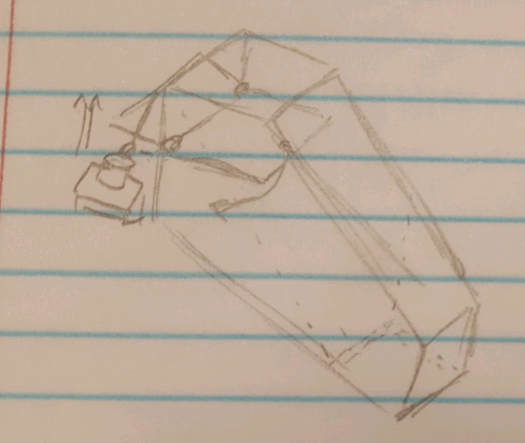
\includegraphics[height=10cm]{Slide.png}}\end{center}
    The slide mechanism would have a sloped platform that would guide the package down into a hole at the bottom. However, there would also exist a separate platform that is kept straight to initially place the package onto. This tilt-able platform would work similarly to a seesaw. One one side, the platform is kept in tension with a motor and string, while on the other side of the fulcrum, the object is placed. Once the object will want to be dropped, the motor would release the tension on the string and uncurl itself, to let the platform fall flat onto the sloped platform beneath simply from the weight of the package. The motor would then be able to retract the string and tighten the platform in a horizontal position again.
    
   \begin{center} Figure2 {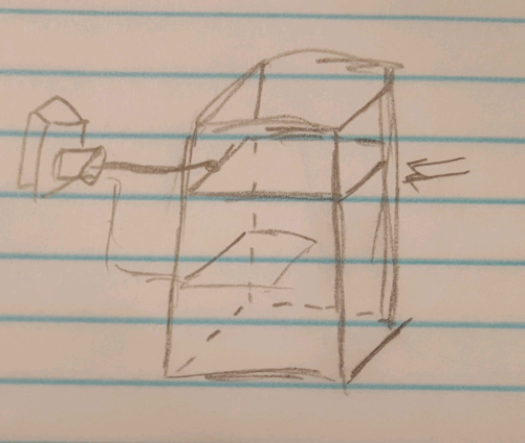
\includegraphics[height=10cm]{DropChute.png}}\end{center}
    The drop chute mechanism would have a tower like design with openings on the top and bottom in which there is a slit on one of the sides to insert a horizontal platform. The package would be placed onto this horizontal platform. Then, the horizontal platform would be pulled out by the motor when the drop is initiated and the floor would slowly be pulled out by the motor from under the package, allowing it to drop down. Further designs were created with multiple floors of different lengths, allowing for multiple deliveries before restocking, but have not been further tested. 
    
    \begin{center}Figure3 {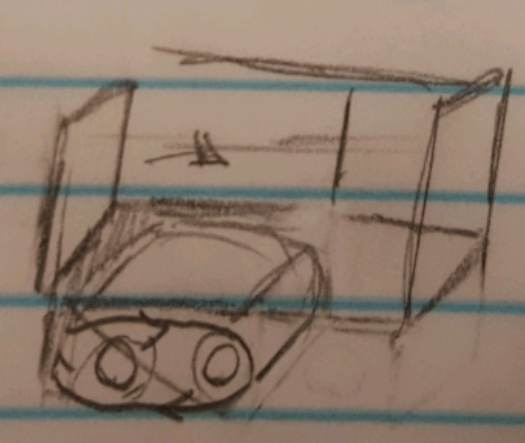
\includegraphics[height=10cm]{Conveyor.png}}\end{center}
    The conveyor mechanism would have a platform encompassing two rotating motors allowing it to move when the motors do. In this way, the package can move on the platform as the floor moves below it and have it fall into a hole at one end. While this design seemed to be the most complicated with two motors, it also allowed for multiple deliveries before being restocked. 

\subsection{Pugh Matrix}
    During the experimental phase of the dropping mechanism, the group began to use a Pugh Matrix to try and quantify the qualities of each of the mechanisms. Overall, we looked to grade our designs based on specific criteria which was implemented from stakeholder beliefs and the group's personal expertise. In order to find the strongest contender, the mechanisms were graded for: Material Cost, Ease of Construction(and Ease for Technicians to Fix), Functionality, and Ability to Hold Multiple Packages. 
    \newpage
    \begin{center}Table1 {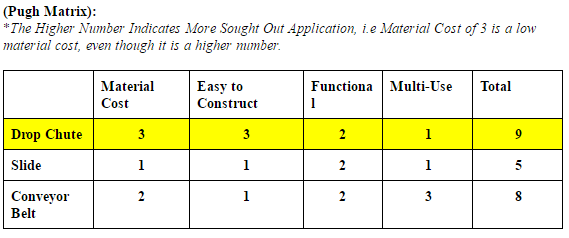
\includegraphics[width=\textwidth]{PughMatrix.png}}\end{center}

    After a thorough analysis, the drop-chute mechanism was chosen to be the one that best fits the needs of the stakeholders and robot. The group believed that the ease of construction and lower material costs would ultimately bring more benefit to the companies than a multi-use functionality. Due to lower costs and complexity, these robots could be mass produced to solve the issue of having to restock for each rescue. Finally, while the slide seemed like a strong idea, there was a lot of unknown surrounding the seesaw technique used and so the idea was dropped for a stronger functional mechanism design. 

\section{Proposed Technical Design}
\subsection{Context Diagram}
A Context Diagram was created to better understand the flow of usage with the robot. The USRR context diagram shows as a whole, all the inputs and outputs from/to external factors when using and creating the robot. In this case, we took into account all many of the stakeholders and tried to understand how each of them would be using the robot.
 \begin{center}{Figure5 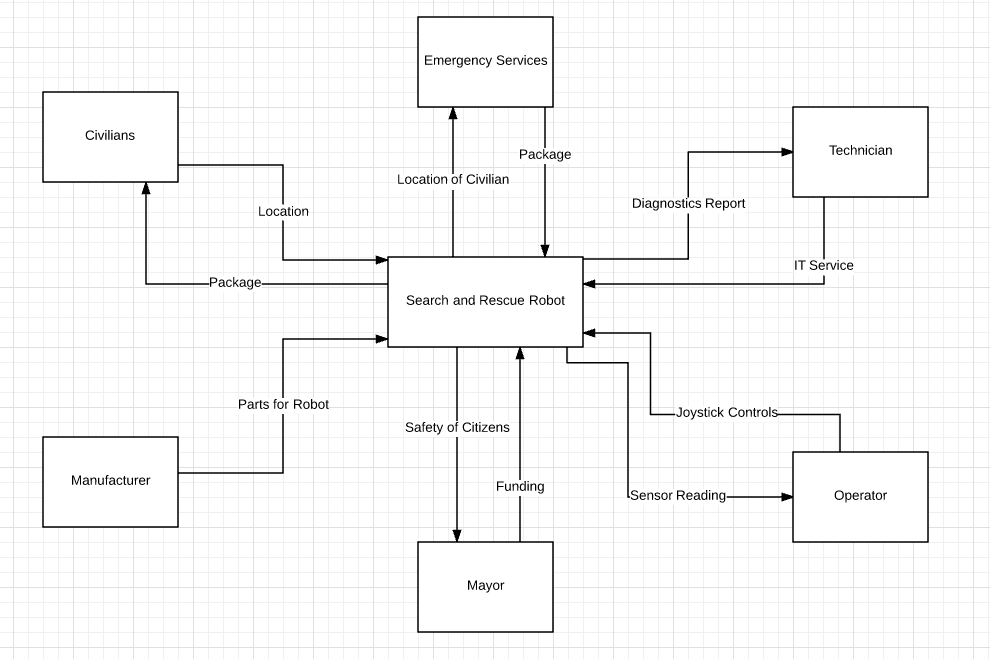
\includegraphics[width=\textwidth]{ContextDiagram.png}}\end{center}

\subsection{Use Cases}
A use case is a list of actions or event steps, typically defining the interactions between a role and a system, to achieve a goal. In this case, the operator, physical robot and software all interact to make the USR Robot fully functional to help the citizens in need. Below, the group has illustrated the way each of the roles interacts with one another in order to successfully use the robot. The Use Cases were split between locating the injured civilian and separately giving the package to the civilian as two different use cases. The search case shows how each of the robot's components will function to try and find the civilian while the drop mechanism use case shows how the robot will be interacted with to release its package to the civilian in need.
    \newpage
    Search Use Case:
    \begin{center}{Figure6 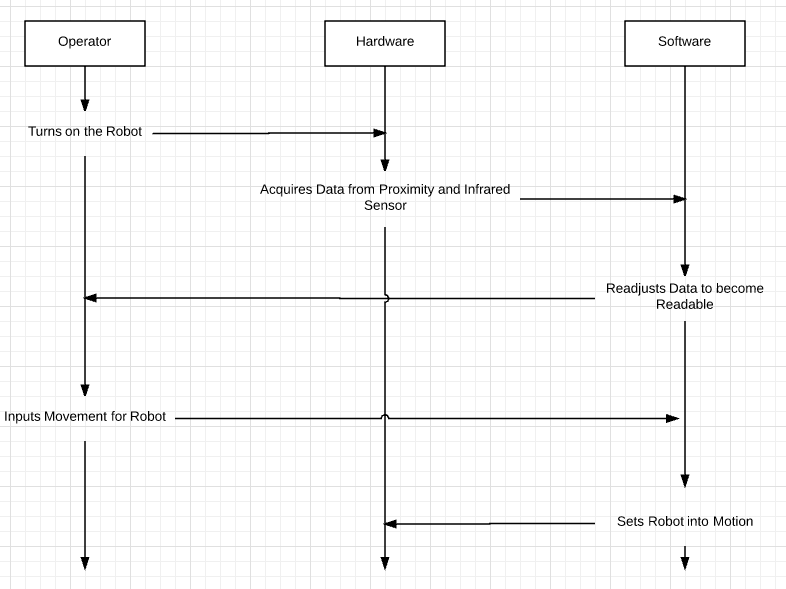
\includegraphics[width=\textwidth]{SearchCase.png}}\end{center}
    
    \newpage
    Drop Mechanism Use Case:
    \begin{center}{Figure7 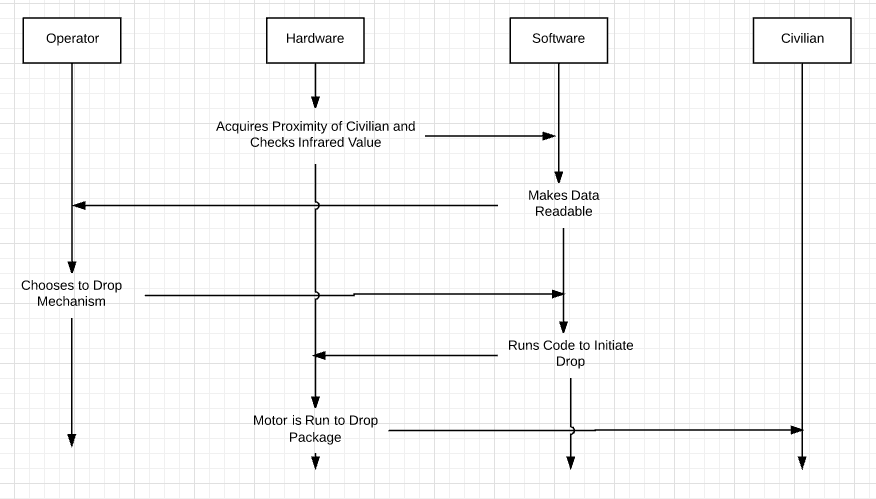
\includegraphics[width=\textwidth]{DropCase.png}}\end{center}
    
\subsection{Conceptual Design}
Initially the robot was developed on top of a sub-assembled chassis, and therefore many conceptual designs consisted of building onto the existing sub-assembly component of the robot. As a major part of the robot's mission, the drop mechanism was conceptualized and previously experimented with to try and create the strongest design possible. After determining which drop mechanism would be used, a SolidWorks model was drafted in order to finally bring the idea to life with measurements and a visual model. This model was used during the construction process of the prototype for measurements and placement of elements together. Below the original SolidWorks design is displayed. The design consisted of a drop chute to place the package and a slit to place a horizontal floor for the package to sit on. A separate structure was built on top of the robot to house the motor which, level with the slit, would be able to pull the horizontal floor from underneath the package and let it fall down.
    
    \begin{center}{Figure8 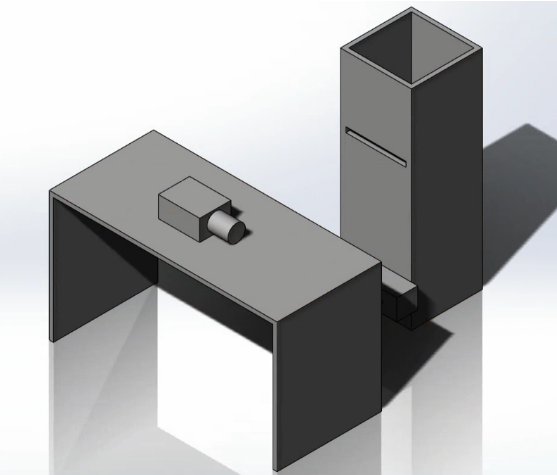
\includegraphics[width=\textwidth]{Solidworks.png}}\end{center}
    
\subsection{Current Development Images}
Here are a few pictures of the robot currently in development to help further explain the ideas above in real life model. A cleanup of wiring still must be made, along with the creation of the raised platform for the drop motor to sit on. However, at the moment all pieces seen are functional, including movement, drop mechanism, and sensor readings.

\begin{center}{Figure9 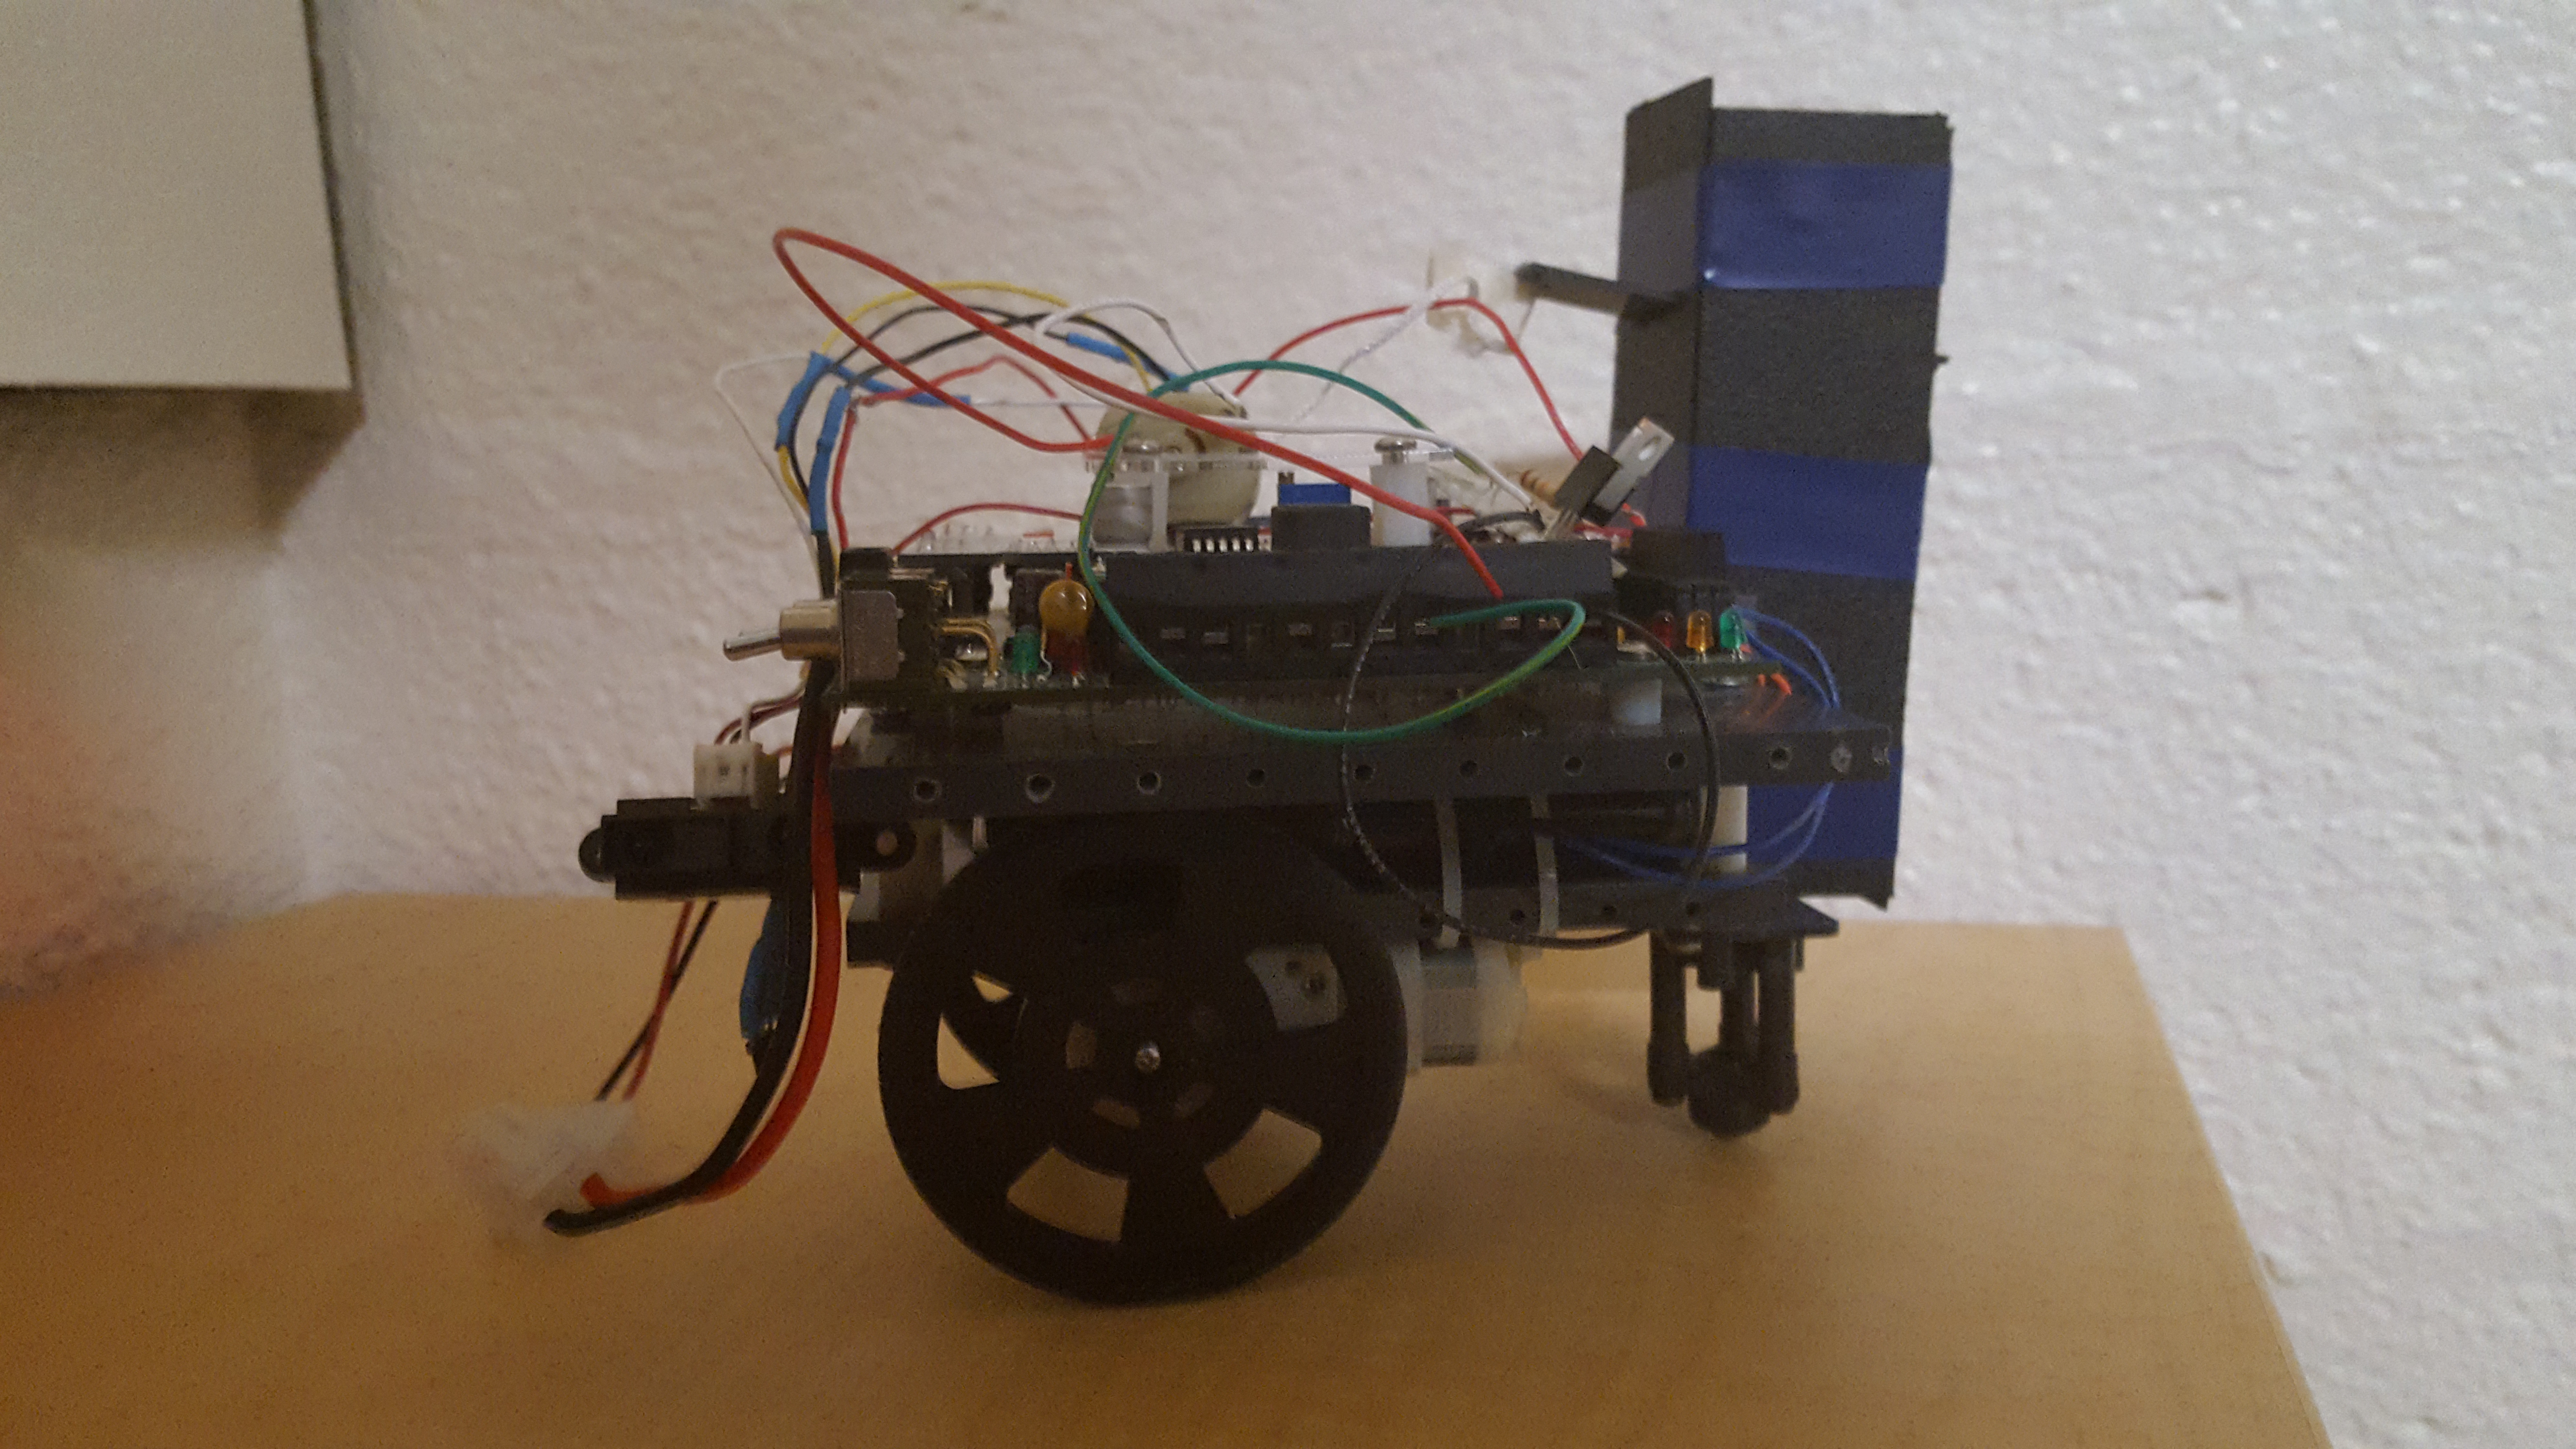
\includegraphics[width=\textwidth]{RobotSide.jpg}}\end{center}
\begin{center}{Figure10 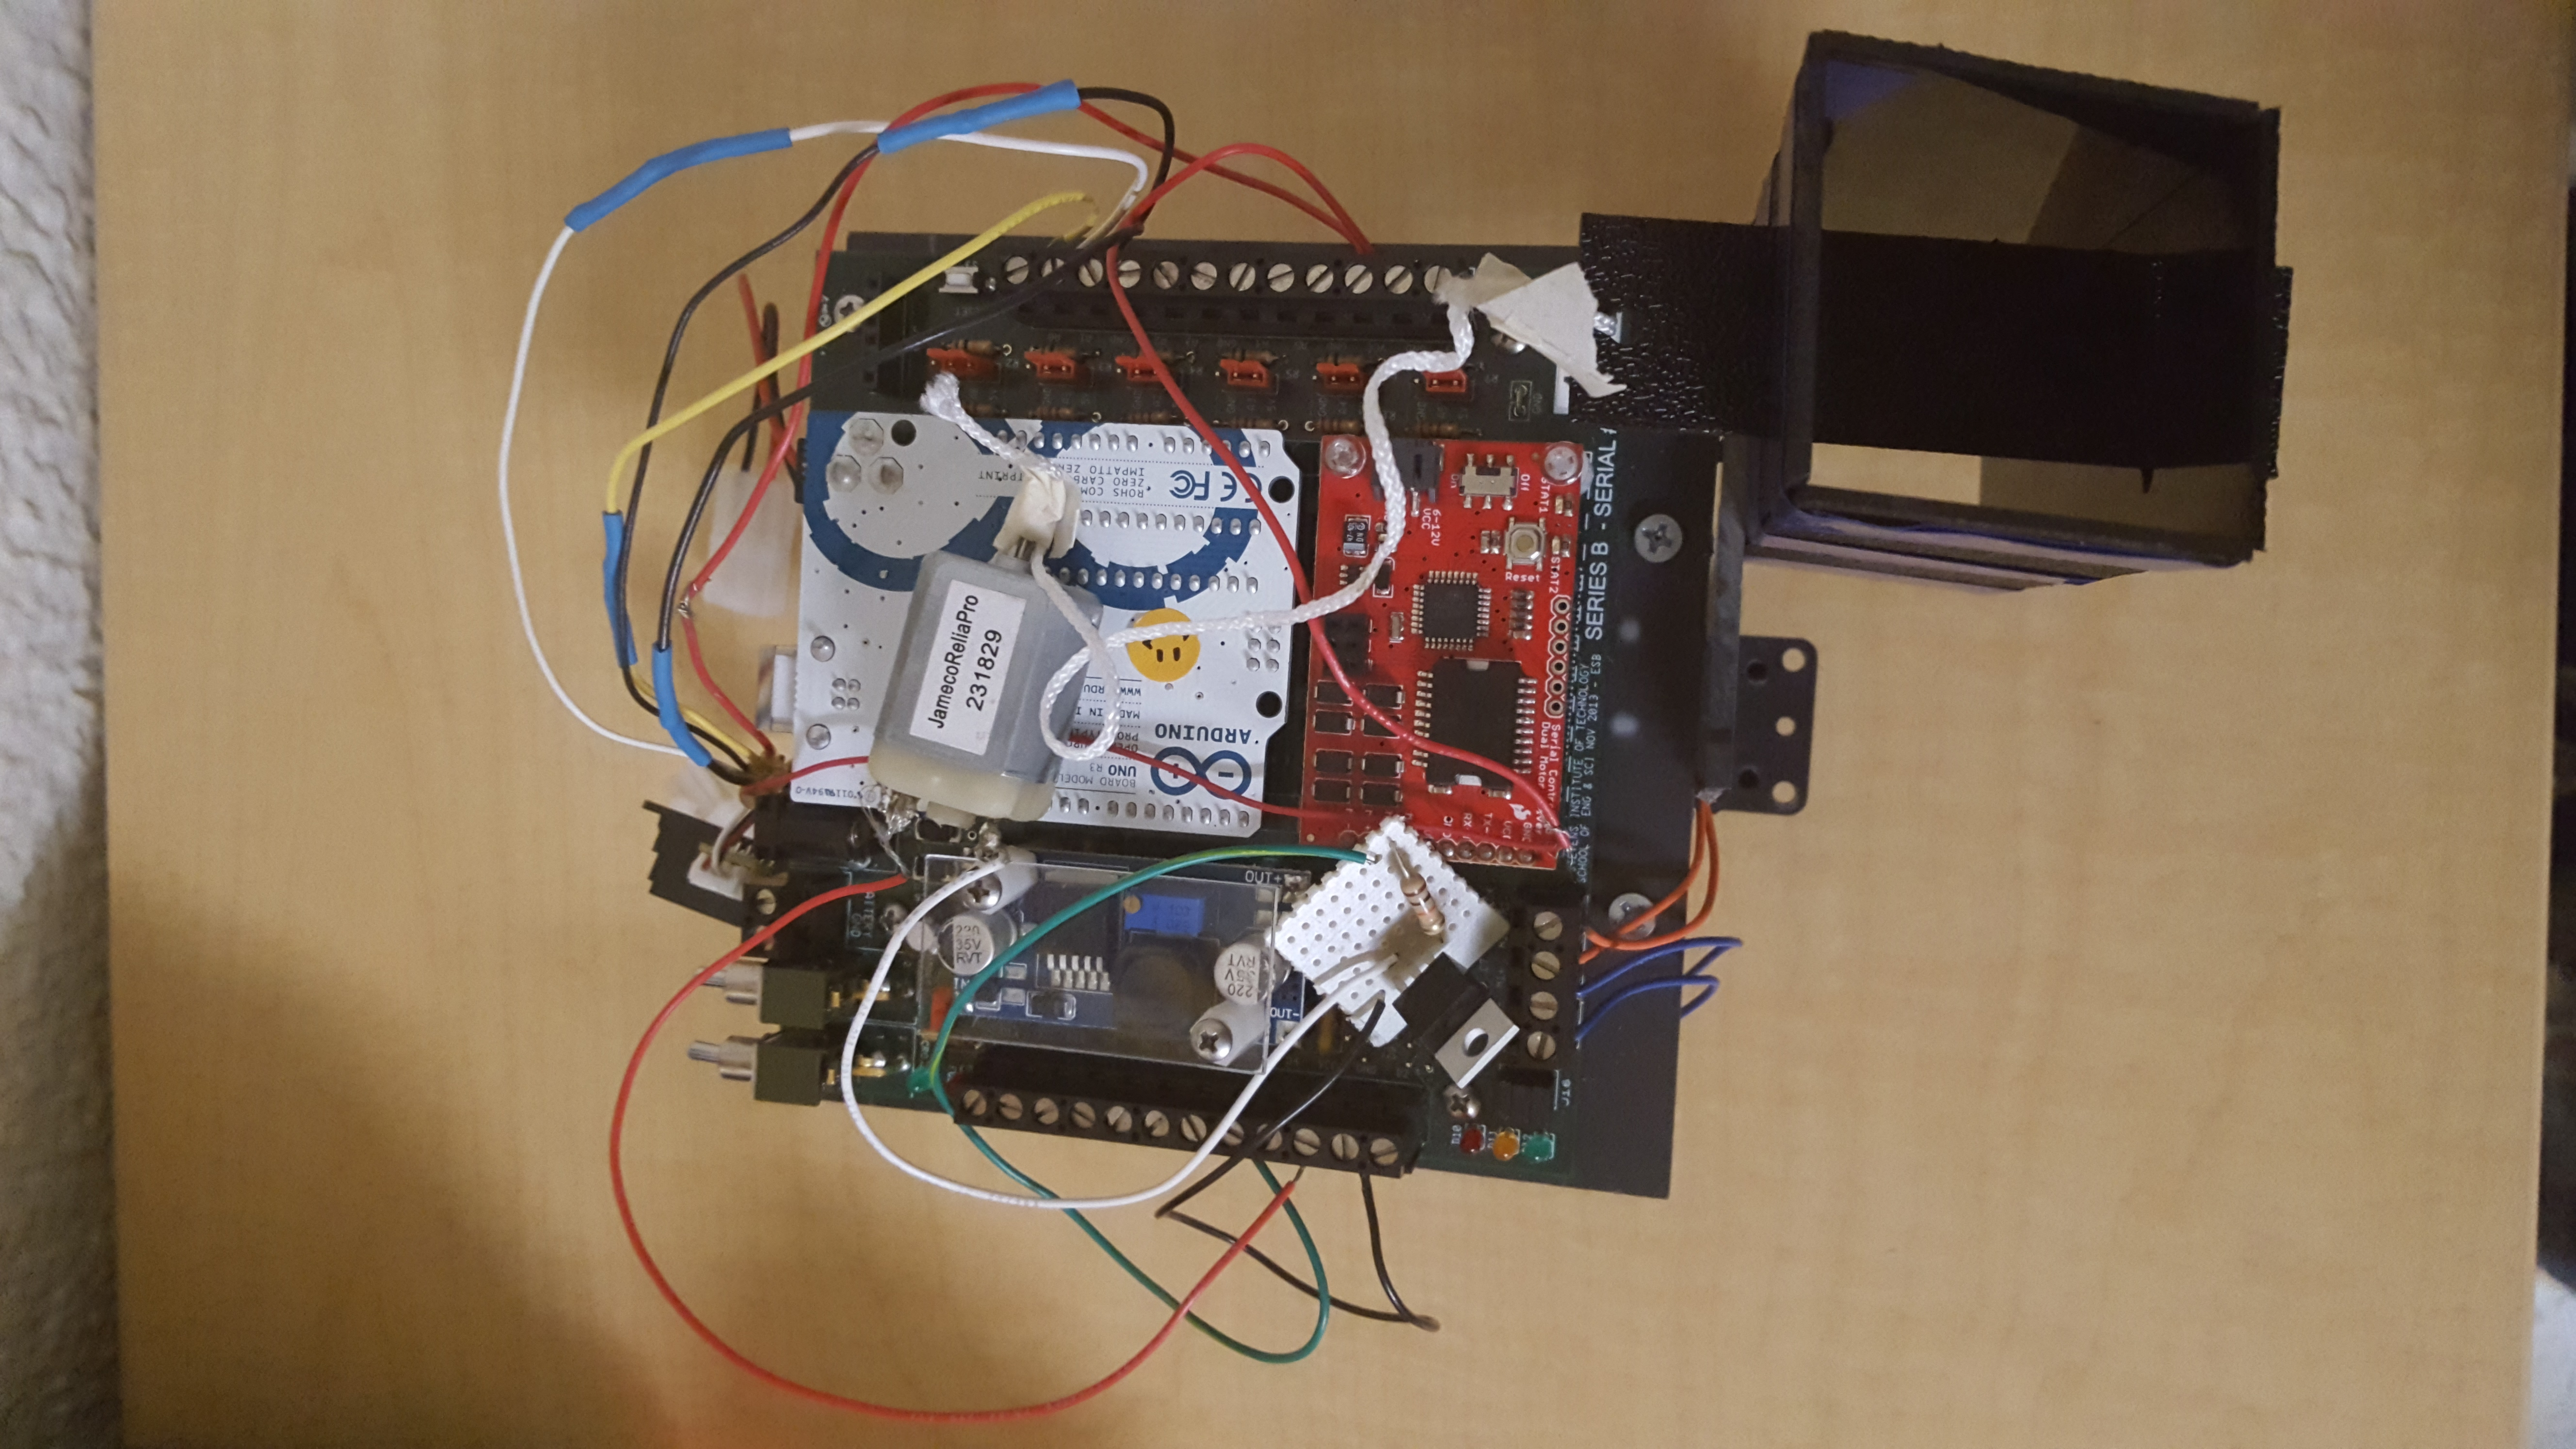
\includegraphics[width=\textwidth]{RobotTop.jpg}}\end{center}

\newpage
\subsection{Block Diagram and Data Flow}
    In order to help understand the flow of actions and coding, a block diagram was created to model the flow of data throughout the trials. This block diagram helped visualize how the different parts of the robot interacted in a more fluid motion and helped with breaking up and positioning separate coding subsections.
     \begin{center}{Figure11 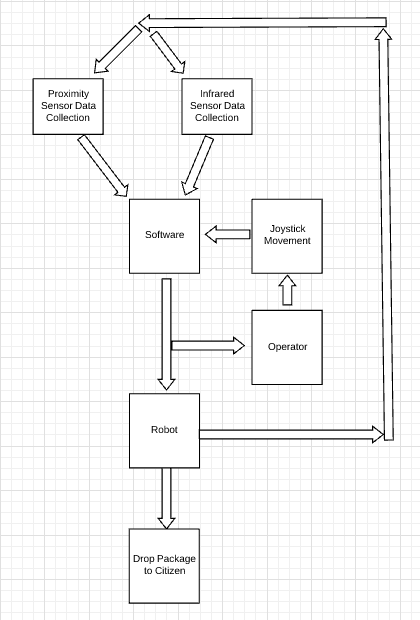
\includegraphics[]{DataFlow.png}}\end{center}
     
\subsection{Software Flowchart}    
A separate software flowchart was used to help model, more specifically, how the data would flow through the trial and showed when the robot would look to answer if-statements and deviate to different paths based on its answers. This allowed our robot to more dynamically work based on inputs and outputs from the operator and sensors/joystick. Thanks to the visualization of the inputs that would be received for movement, the group decided to work with a boolean array using binary to adjust integers into different cases. Thresholds were set for indications of if the joystick was pushed far enough to register movement in that direction. The boolean array later allowed us to combine multiple options by converting the array into an integer value, by converting binary to integers using the powers of 2. This will be further explained in the software section.
    \begin{center}{Figure12 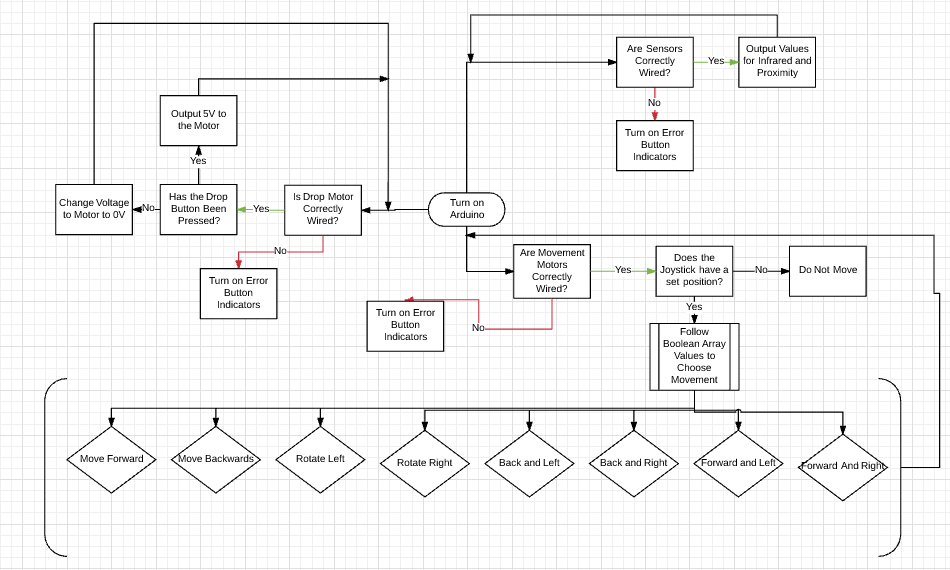
\includegraphics[width=\textwidth]{SoftwareFlowchart.png}}\end{center}
    
\subsection{Materials}
Throughout the creation of the USRR, a list of materials was kept in order to understand how complex the robot has become and how much it would cost financially to build. Here is a list of all the materials used:

\begin{itemize}
    \item Chassis Sub-assembly x1
    \item Arduino Microprocessor Board x1
    \item AC Wall Adapter x1
    \item Battery x1
    \text Battery Connection Cable x1
    \item USB A-B Cable x1
    \item Gray PVC (6"x6") x2
    \item Dark Gray Plastic (12"x12") x1
    \item Infrared Sensor x1
    \item Proximity Sensor x1
    \item Arduino Mounting Package x1
    \item Transistor x1
    \item 10k Ohm Resistor x1
    \item Assortment of Wires (Multiple Colors)
    \item Screws x8
    \item Motors x3 (2 are part of the sub-assembly)
    \item Joystick
\end{itemize}

\subsection{Sensor Data}
While each of the sensors was purchased off the shelf, the data collected from each of them needed to be calibrated to be readable by the operator in correct units. The LabView program was able to correctly calibrate the infrared sensor to graph data in volts, while the proximity sensor was calibrated to give back a reading in centimeters away from the sensor. The calculations can be seen in the LabView Block Diagram further in the proposal. (See Block Diagram in the Appendix).

\subsection{LabView Front Panel}
When constructing the front panel, the group had the operator in mind, as well as the technician to make the robot a simple process both in collecting data, but also in displaying data from sensors and button presses. 
\begin{center}{Figure13 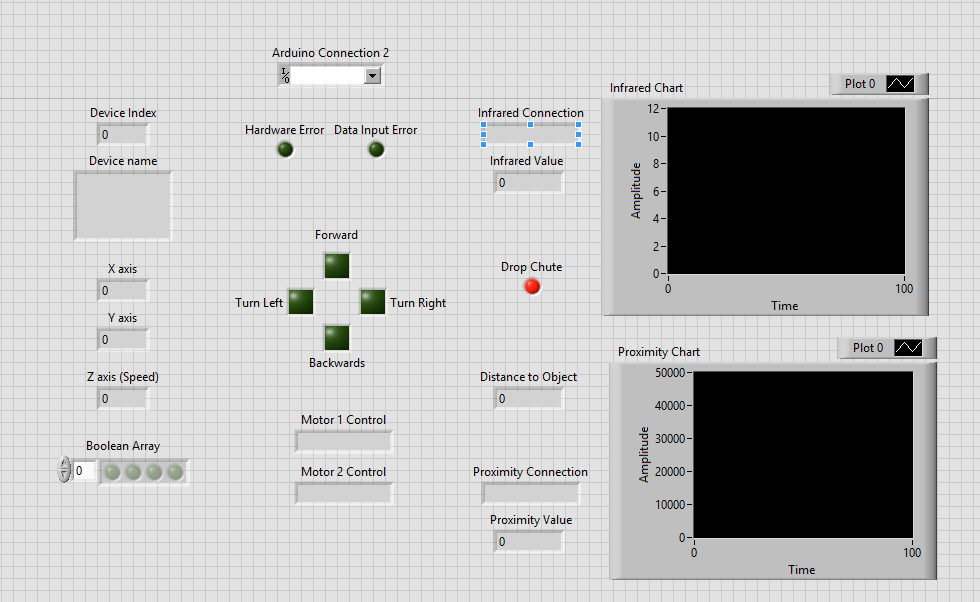
\includegraphics[width=\textwidth]{FrontPanel.png}}\end{center}
\begin{itemize}
    \item On the left side of the screen the device index allows technicians to evaluate the control (joystick) and see if it is correctly being read by the LabView Program. When correctly connected the Device Index will display the port number that the device is connected to, and the Device Name should show the name of the device that is connected to control movement.
    \item Under the device index and name, the raw x,y, and z axis data are displayed to show raw input from the joystick, in case some changes need to be made to thresholds for movement. These values also help the operator visually understand how big or small of a movement must be made on the joystick before to move the robot.
    \item The Boolean array at the bottom, as well as the directional buttons in the middle of the display help associate the threshold values to movements. In this case, the operator can see that when the joystick is moved forward, the forward LED will light up, unless there is an error. This design helps both with error checking and operator visualization. If the robot's forward LED is on, but the robot is not moving forward then the code written must be changed. From the operator's point of view, the LEDs allow him to focus his attention on the LabView Front Panel than on the joystick.
    \item On the Right side, Infrared values and proximity values are shown both as single values and in graph form to help the operator decide on movement. While the singular values are all that are necessary to create a decision, the implementation of the graph helps the operator visualize the sensors data over time. For example, by hooking up the proximity sensor to a graph, the operator is able to visualize the robot approaching closer or further away from an object. Similarly, he can see spikes in infrared readings, from rotations or movement, without having to remember average values.
    \item An LED was added to associate with the Drop Chute button, which lights green when the drop mechanism is initiated. This can be used both as an indicator and for error checking, to know if the error coming from the code is made from the code itself, or from hardware malfunctions.
    \item Extra Error checking values have also been left on the Front Panel, including the messages sent to the Arduino itself for movement displayed in "Motor 1 Control and Motor 2 Control" as well as LEDs on top to check if the Arduino is correctly associating with the LabView Program. These help mostly the technician associate exactly what the Arduino is being sent in string form in order to change things like speed, analog ports, or motor ports.
\end{itemize}

\subsection{LabView Block Diagram}
Below are separate sections of the block diagram, organized according to their function. Each diagram has its own function to do, and all of the functions are found inside a large while statement to make them continuously run and keep receiving inputs from the joystick. 

\begin{center}{Figure14 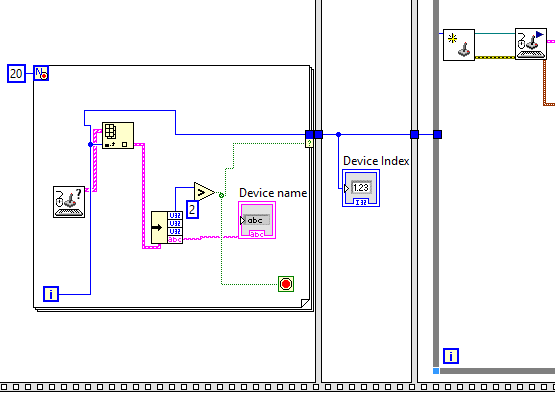
\includegraphics[]{JoystickVI.png}}\end{center}
Figure 14 shows the joystickVI which has been imported into the block diagram in order to gain values from the joystick. The joystick allows multiple button presses to be registered as well as values for x,y,z rotation and transformation. However, the team decided that not all of these are needed and cleaned up the amount that we used to one button and the x,y,z transformations. 

\begin{center}{Figure15 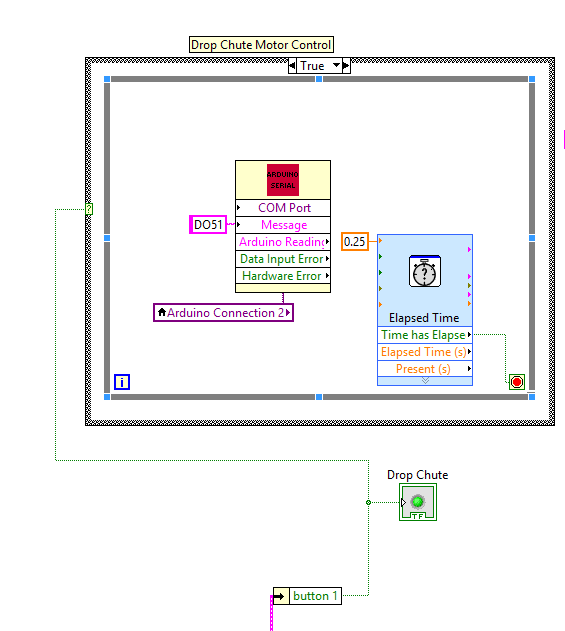
\includegraphics[height=10cm]{DropChute1.png}}\end{center}
\begin{center}{Figure16 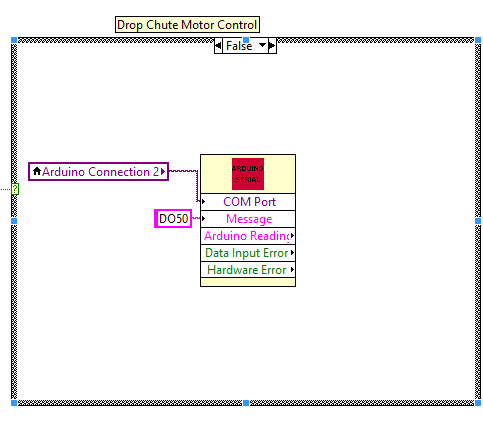
\includegraphics[height=10cm]{DropChute2.png}}\end{center}

Figure 15 and 16 show the code to make the drop mechanism work. In this case, button 1 from the joystick is registered and converted into a boolean value as either pressed or not pressed. When pressed the button lights up and the true statement goes through, otherwise, the false statement goes through. In the true statement, the group makes sure to send a current through the motor to increase the voltage, causing it to turn on and spin retracting the platform with it and allowing the payload to be delivered. The Elapsed Time function is used in a while loop to limit the current running through the solenoid to 1 second pulses in order to prevent the hardware from overheating due to too many function calls. When false, the digital output the motor is connected to is set to 0V and therefore it does not run. 
\\\\We decided we only needed to make a one directional motor in order to simplify the coding process and the technical issues involved. Since the group only needed a platform to be jerked out from under the payload, only one direction was needed. In order to reset the USRR for another delivery, manual reset of the platform needs to be made. Timed, this action only takes 10 seconds to do at most.

\begin{center}{Figure17 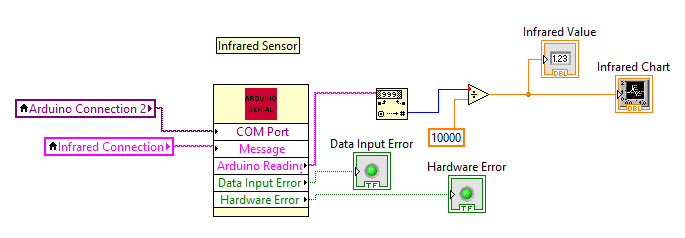
\includegraphics[width=\textwidth]{InfraRedSensor.png}}\end{center}
In Figure 17 the robot likewise acts as a DAQ device and collects data from the Proximity Sensor. There is also a conversion equation to change the raw values of the data and changing into readable as a unit of voltage. This value is then displayed and graphed for the operator to use to be more successful in his/her operation of the USRR to the civilian in need.

\begin{center}{Figure18 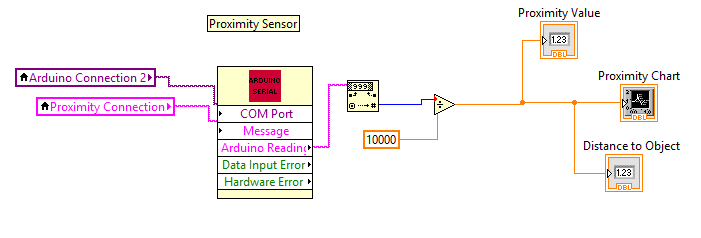
\includegraphics[width=\textwidth]{ProximitySensor.png}}\end{center}
In Figure 18 the robot looks to act as a DAQ device and collect the data from the proximity sensor, output it as a calibrated value that can be read as a distance and the graph the value. At the moment, the proximity sensor displays data as a unit of voltage, and further testing must be done to find the equation to convert into cm distance from the target. The graph is beneficial in assisting the operator in making decisions on movement input by looking at the changes over time in the sensor's data.

\begin{center}{Figure19 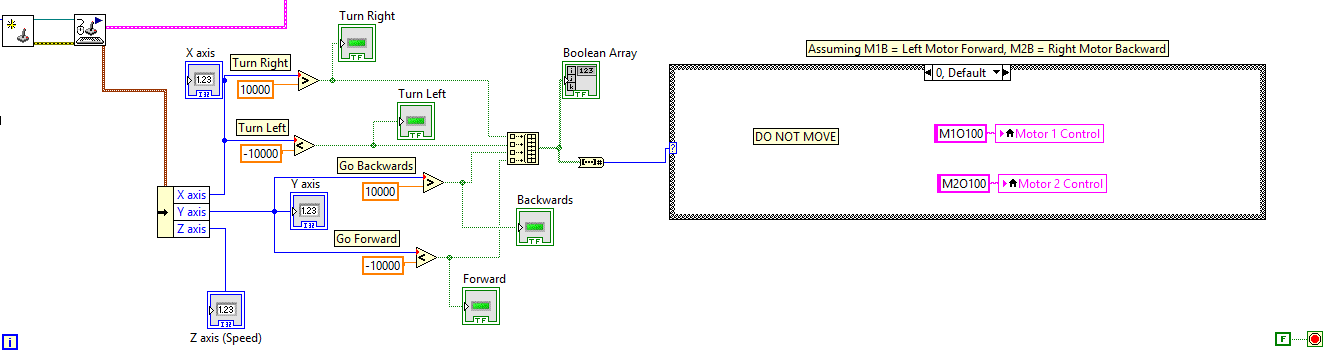
\includegraphics[width=\textwidth]{MotorMovement.png}}\end{center}
The motor movement was created using a threshold approach from the values taken from the joystick. The joystick device itself was able to send values for x-axis, y-axis, and z-axis transformations. By unbundling these values and comparing them to set thresholds, the group could decide at what point the robot would begin to move from the movement of the joystick.
\\\\Each axis was individually tested around the thresholds of 0 and 10000 and -10000 and 0; If the value was above 10000, we know they wanted a positive change in that axis (move forward or turn right) because of +x and +y values. Likewise, if the value was under -10000, the user would input the opposite of the positive change (move backwards or turn left). Values that were between -10000 and 10000 were considered to be too small and defaulted to no motion.
\\\\To gain 8 different motion types, each of these thresholds were tested and converted into a true/false boolean. This boolean was later put into a boolean array and converted into an integer value. To further explain: If a value was above 10000 in the x-axis, the true statement would appear for that boolean. From first to 4th position the values of each position are \[2^0 , 2^1, 2^2, 2^3\]. Based on binary, these numbers could then be turned back into an integer value.
\\\\If the boolean statement was input that right movement (1st slot) and forward movement (3rd slot) were true and the others were false, the boolean array would read (1010). This converted from binary would become: 
\[1*2^0 + 0*2^1 + 1*2^2 + 0*2^3 = 5\]
Then, a case statement can be made to make the robot move forward and right at the same time. With these binary combinations, 15 different case statements could be made as a maximum value, and so 8 different movements could be displayed for different integer types.
\\\\Only one is shown in the above code, the default. When 0 is received, no movement is made to the robot. Different motor strings were attached to each of the following integers allowing them to all have different types of motor inputs to the Arduino: 
\begin{center}{Figure20 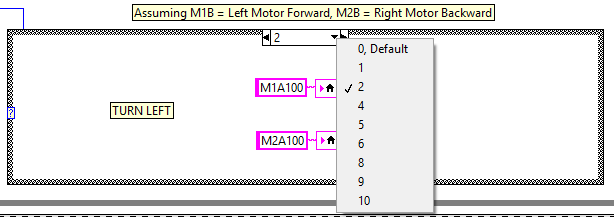
\includegraphics[width=\textwidth]{CaseState.png}}\end{center}


Finally, the full code all together can be seen here:
\begin{center}{Figure21 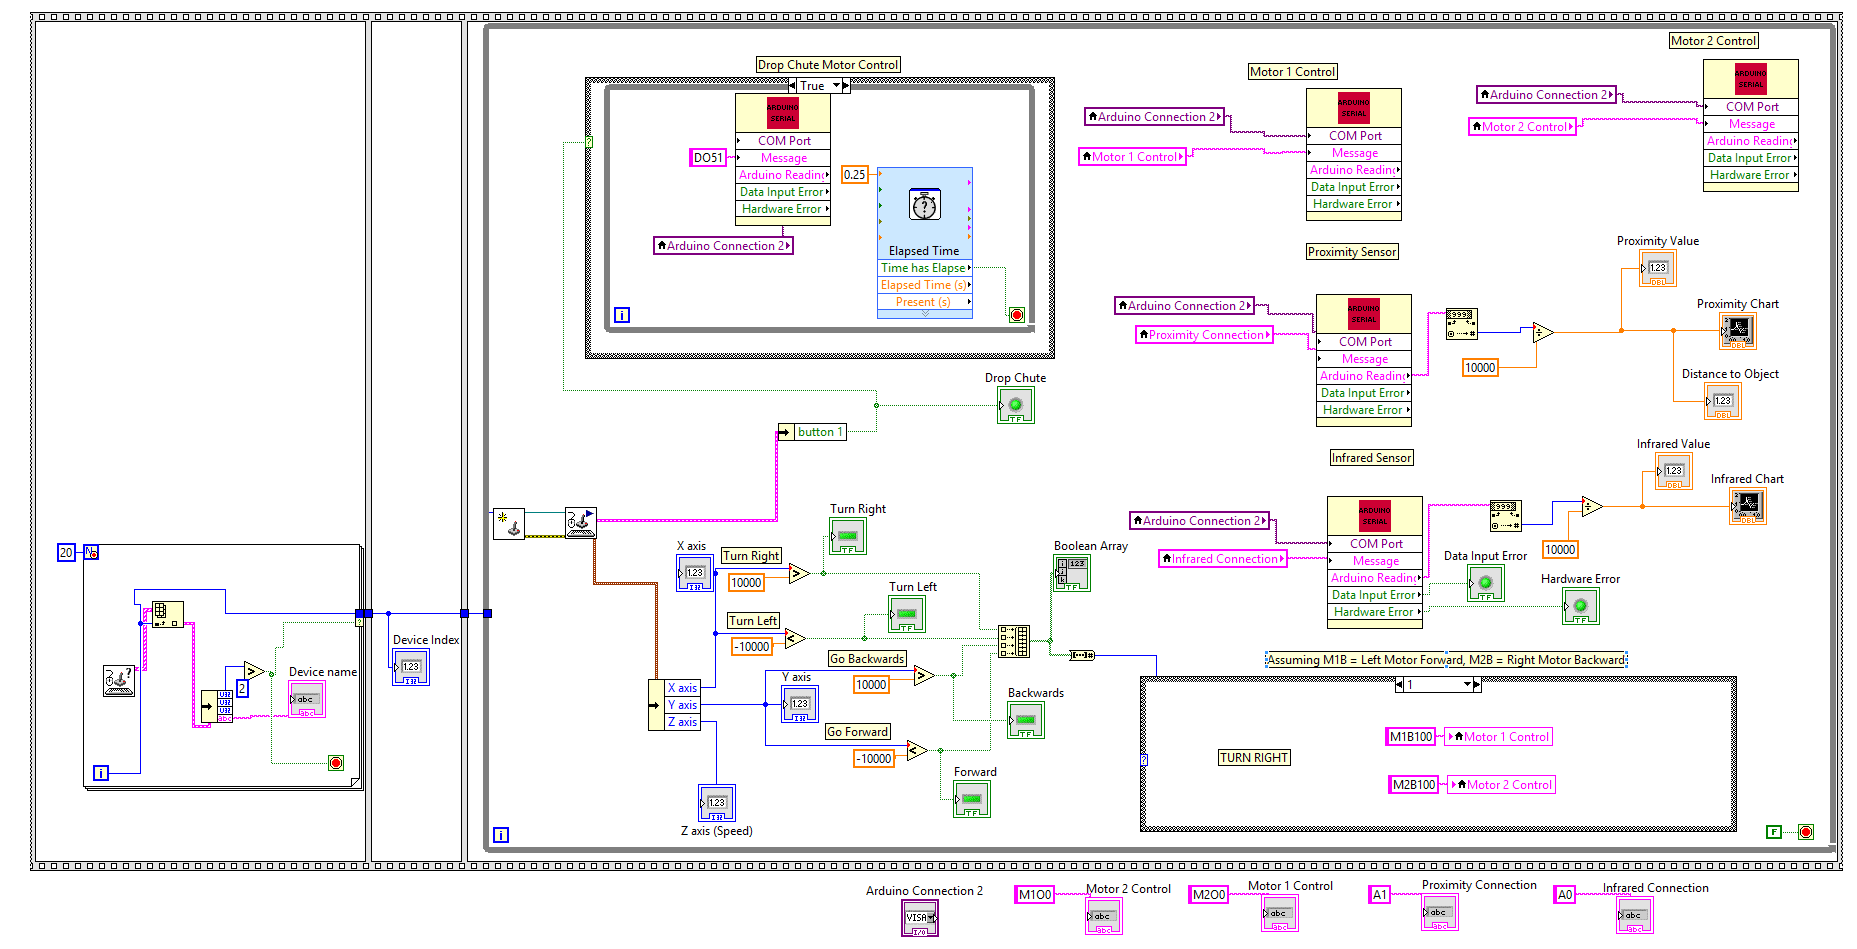
\includegraphics[width=\textwidth]{FullCode.png}}\end{center}


\susection{Proof of Concept}
The group testing and implemented many of the functions of the robot from prior testing and experimentation. First, a separate experiment was made to choose the strongest contender for the drop off mechanism. Later, this was tested through experimentation to work consistently and not have the payload get stuck and not fall through. 
Likewise, the code made for the movement and initiation for the drop off mechanism have all been tested accordingly. The movement of the robot is able to be input and differentiated between say, forward motion and right motion. Likewise, the drop off mechanism is able to be initiated from a button on the joystick. Extra trials are still being run and testing is in full effect. Issues that are being looked at are input lag from the joystick and changing the speed based on the z-axis (throttle) of the joystick. These tests will help the robot move more efficiently and allow for less error when finally applied to the real life situation it is being created for.


\section{Project Plan}
\subsection{Gannt Chart}
In order to keep the group up to date with deadlines and the schedule of the project, a Gannt Chart was used. Each member could look at the Gannt Chart and figure out what needed to be completed by the end of the week.
\begin{center}{Figure22 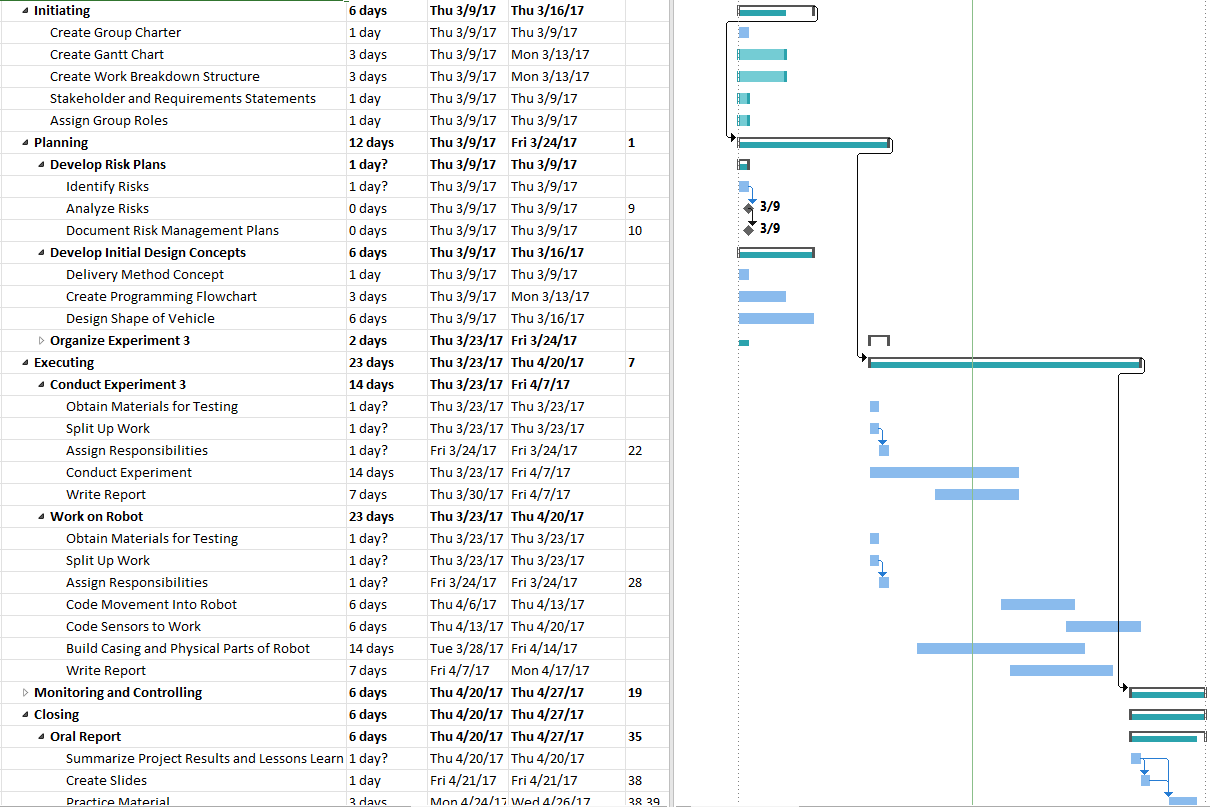
\includegraphics[width=\textwidth]{GanttChart.png}}\end{center}

\subsection{Work Breakdown Structure}

\begin{center}{Figure23 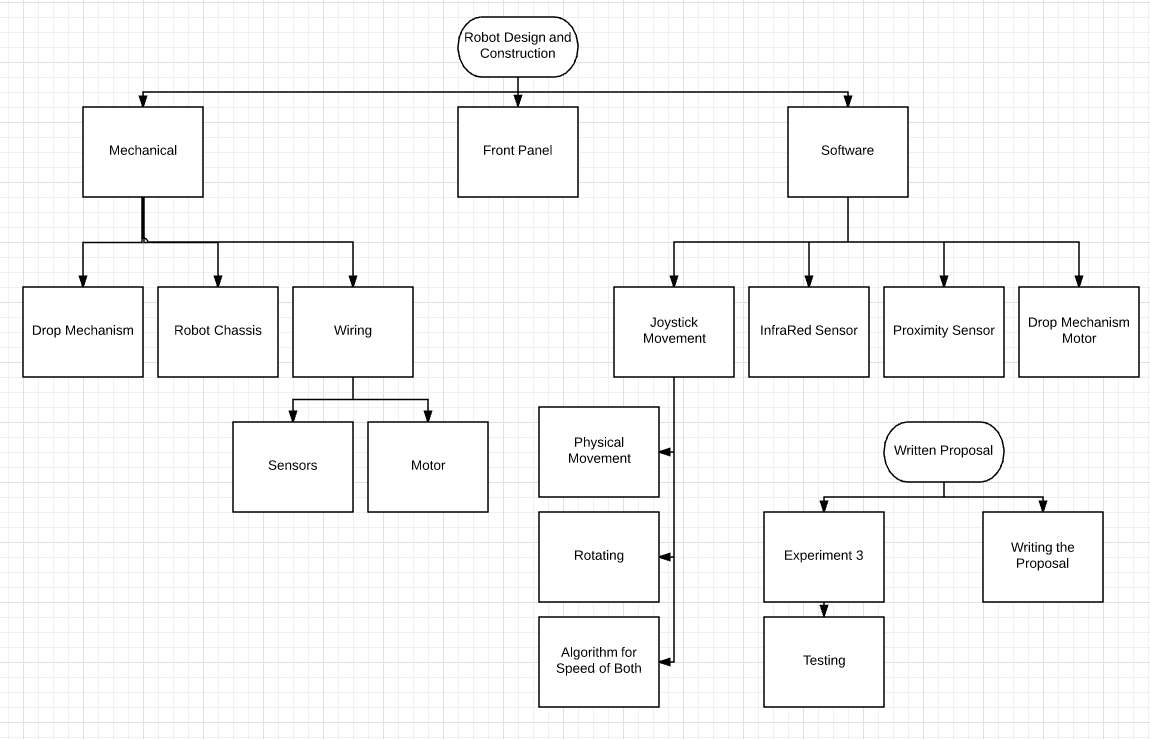
\includegraphics[width=\textwidth]{WorkBreakdown.png}}\end{center}
    A Work Breakdown Structure was created to help organize the separate segments that needed to be completed within the robot design process. Three main features needed to be finished by the end of the process: A physical/mechanically built robot, a functional front panel to use, and software that correctly implemented the front panel. 
    \begin{itemize}
        \item With mechanical construction, the drop mechanism had to be built and tested, the robot needed to have a secure chassis to mount the drop mechanism motor onto and wiring had to be done between all the sensors. In order to properly wire the solenoid, a transistor must be used to ensure that the arduino board would not destroyed by the solenoid.
        \item The front panel had to be constructed to be easy to use and quick to learn for operators. The front panel of LABView was constructed at the same time as the software was being constructed. Furthermore, the front panel needed to easily display the sensor data from the proximity sensor and the infrared sensor.
        \item The software side of the robot had to be made correctly in order to successfully control the robot and make it function as intended. The project was split here between the individual infrared and proximity sensors, as well as the drop mechanism to each work as intended.
        \item The report had to finally be written and our analysis needed to be documented correctly in order to send to the proposal as effectively as possible. The separate experiment to learn about the best drop mechanism and the completed written report were both written. 
    \end{itemize}

\subsection{Team Assignments}
    In order to work clearly and effectively each member of the group was assigned a role as a primary assignment. Each member could help the others out with their designs, but in the end their work needed to be completed on time. Marcin acted as the project manager, scheduling times to meet and assigning roles and projects that would be due next week through the Gantt Chart. He was also head of programming. Daniel helped with creating the Solidworks model and was left in charge of Experiment 3's design and pugh matrix. Anthony was the head mechanical engineer, creating the extra supports around the chassis and the drop down mechanism from supplies in the lab. Each member contributed to writing the report and wiring the robot.

    Furthermore, a Team Charter was drafted in order to have a written document of rules to abide, and its consequences for breaking them: 
    \begin{center}{Figure24 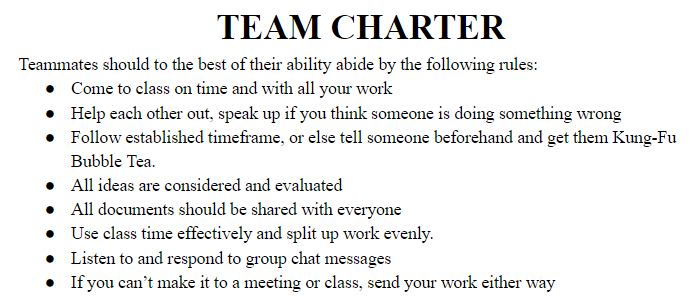
\includegraphics[width=\textwidth]{TeamCharter.png}}\end{center}

\newpage
\section{Financials}
 \begin{center}Figure25 {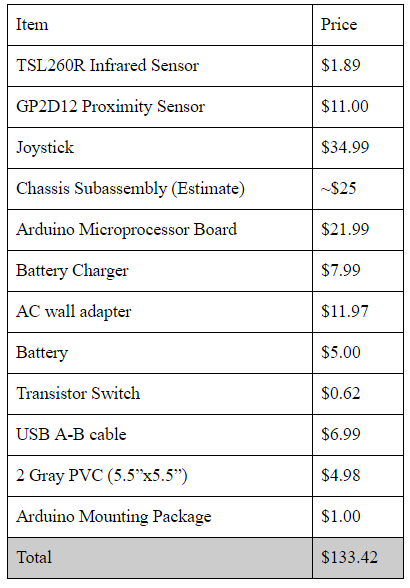
\includegraphics[]{Financials.png}}\end{center}

\newpage
\setcounter{page}{1}
\renewcommand{\thepage}{A-\arabic{page}}
\section{Appendix: Figures and Tables}

\subsection{Figure 1: Slide Design}
\begin{center}{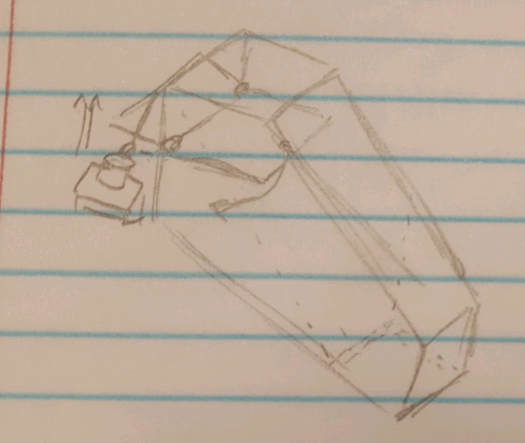
\includegraphics[height=8cm]{Slide.png}}\end{center}

\subsection{Figure 2: Drop Chute Design}
\begin{center}{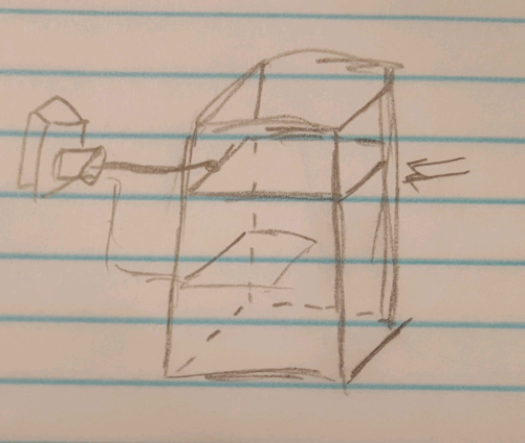
\includegraphics[height=8cm]{DropChute.png}}\end{center}

\subsection{Figure 3: Conveyor Design}
\begin{center}{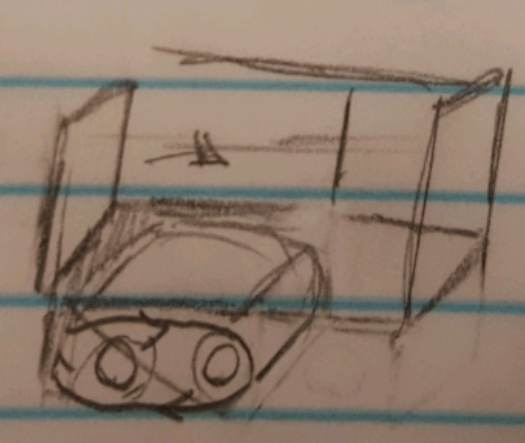
\includegraphics[height=8cm]{Conveyor.png}}\end{center}

\subsection{Figure 4: Pugh Matrix}
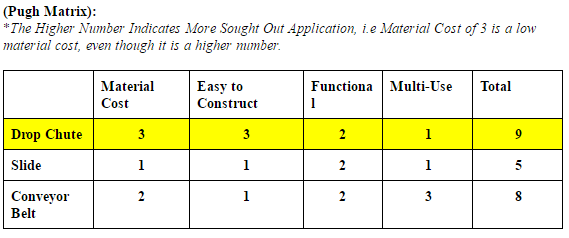
\includegraphics[width=\textwidth]{PughMatrix.png}

\subsection{Figure 5: ContextDiagram}
\begin{center}{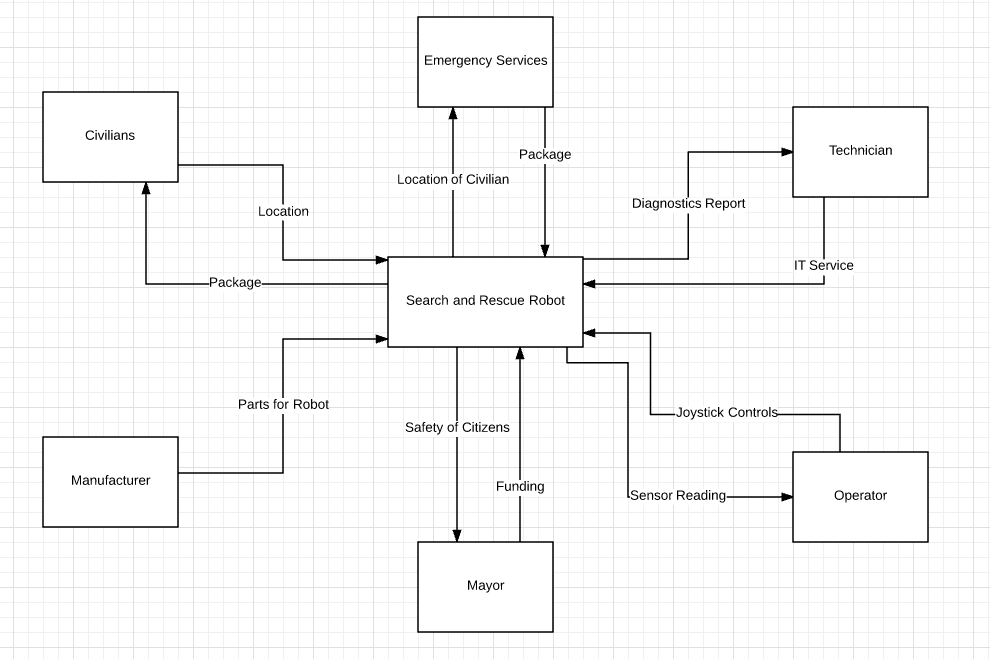
\includegraphics[width=\textwidth]{ContextDiagram.png}}\end{center}

\subsection{Figure 6: Use Cases}
\begin{center}{ 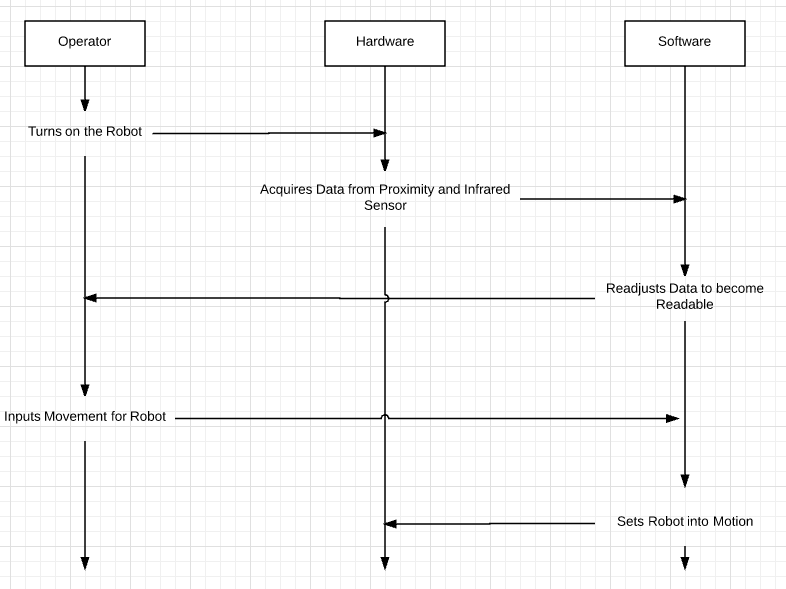
\includegraphics[width=\textwidth]{SearchCase.png}}\end{center}

\subsection{Figure 7: Drop Case}
\begin{center}{ 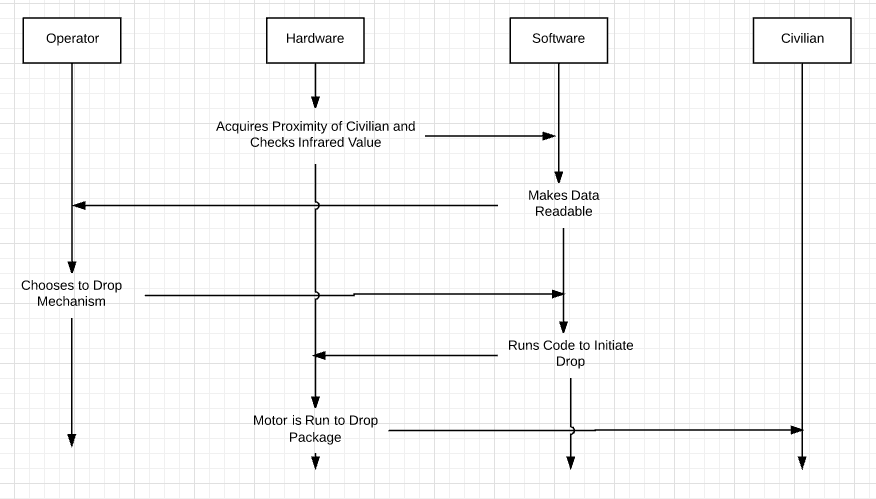
\includegraphics[width=\textwidth]{DropCase.png}}\end{center}

\subsection{Figure 8: SolidWorks Model}
\begin{center}{ 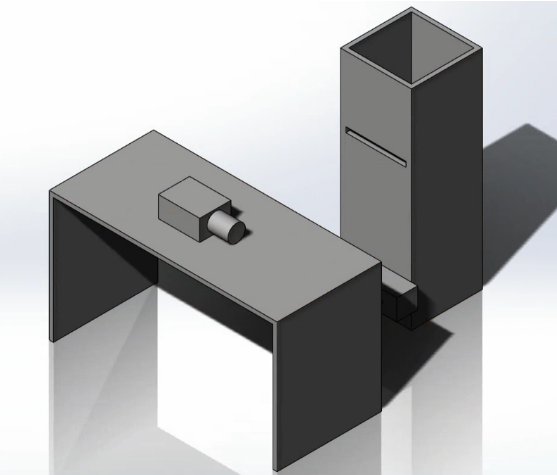
\includegraphics[width=\textwidth]{Solidworks.png}}\end{center}

\subsection{Figure 9: Robot Side}
\begin{center}{ 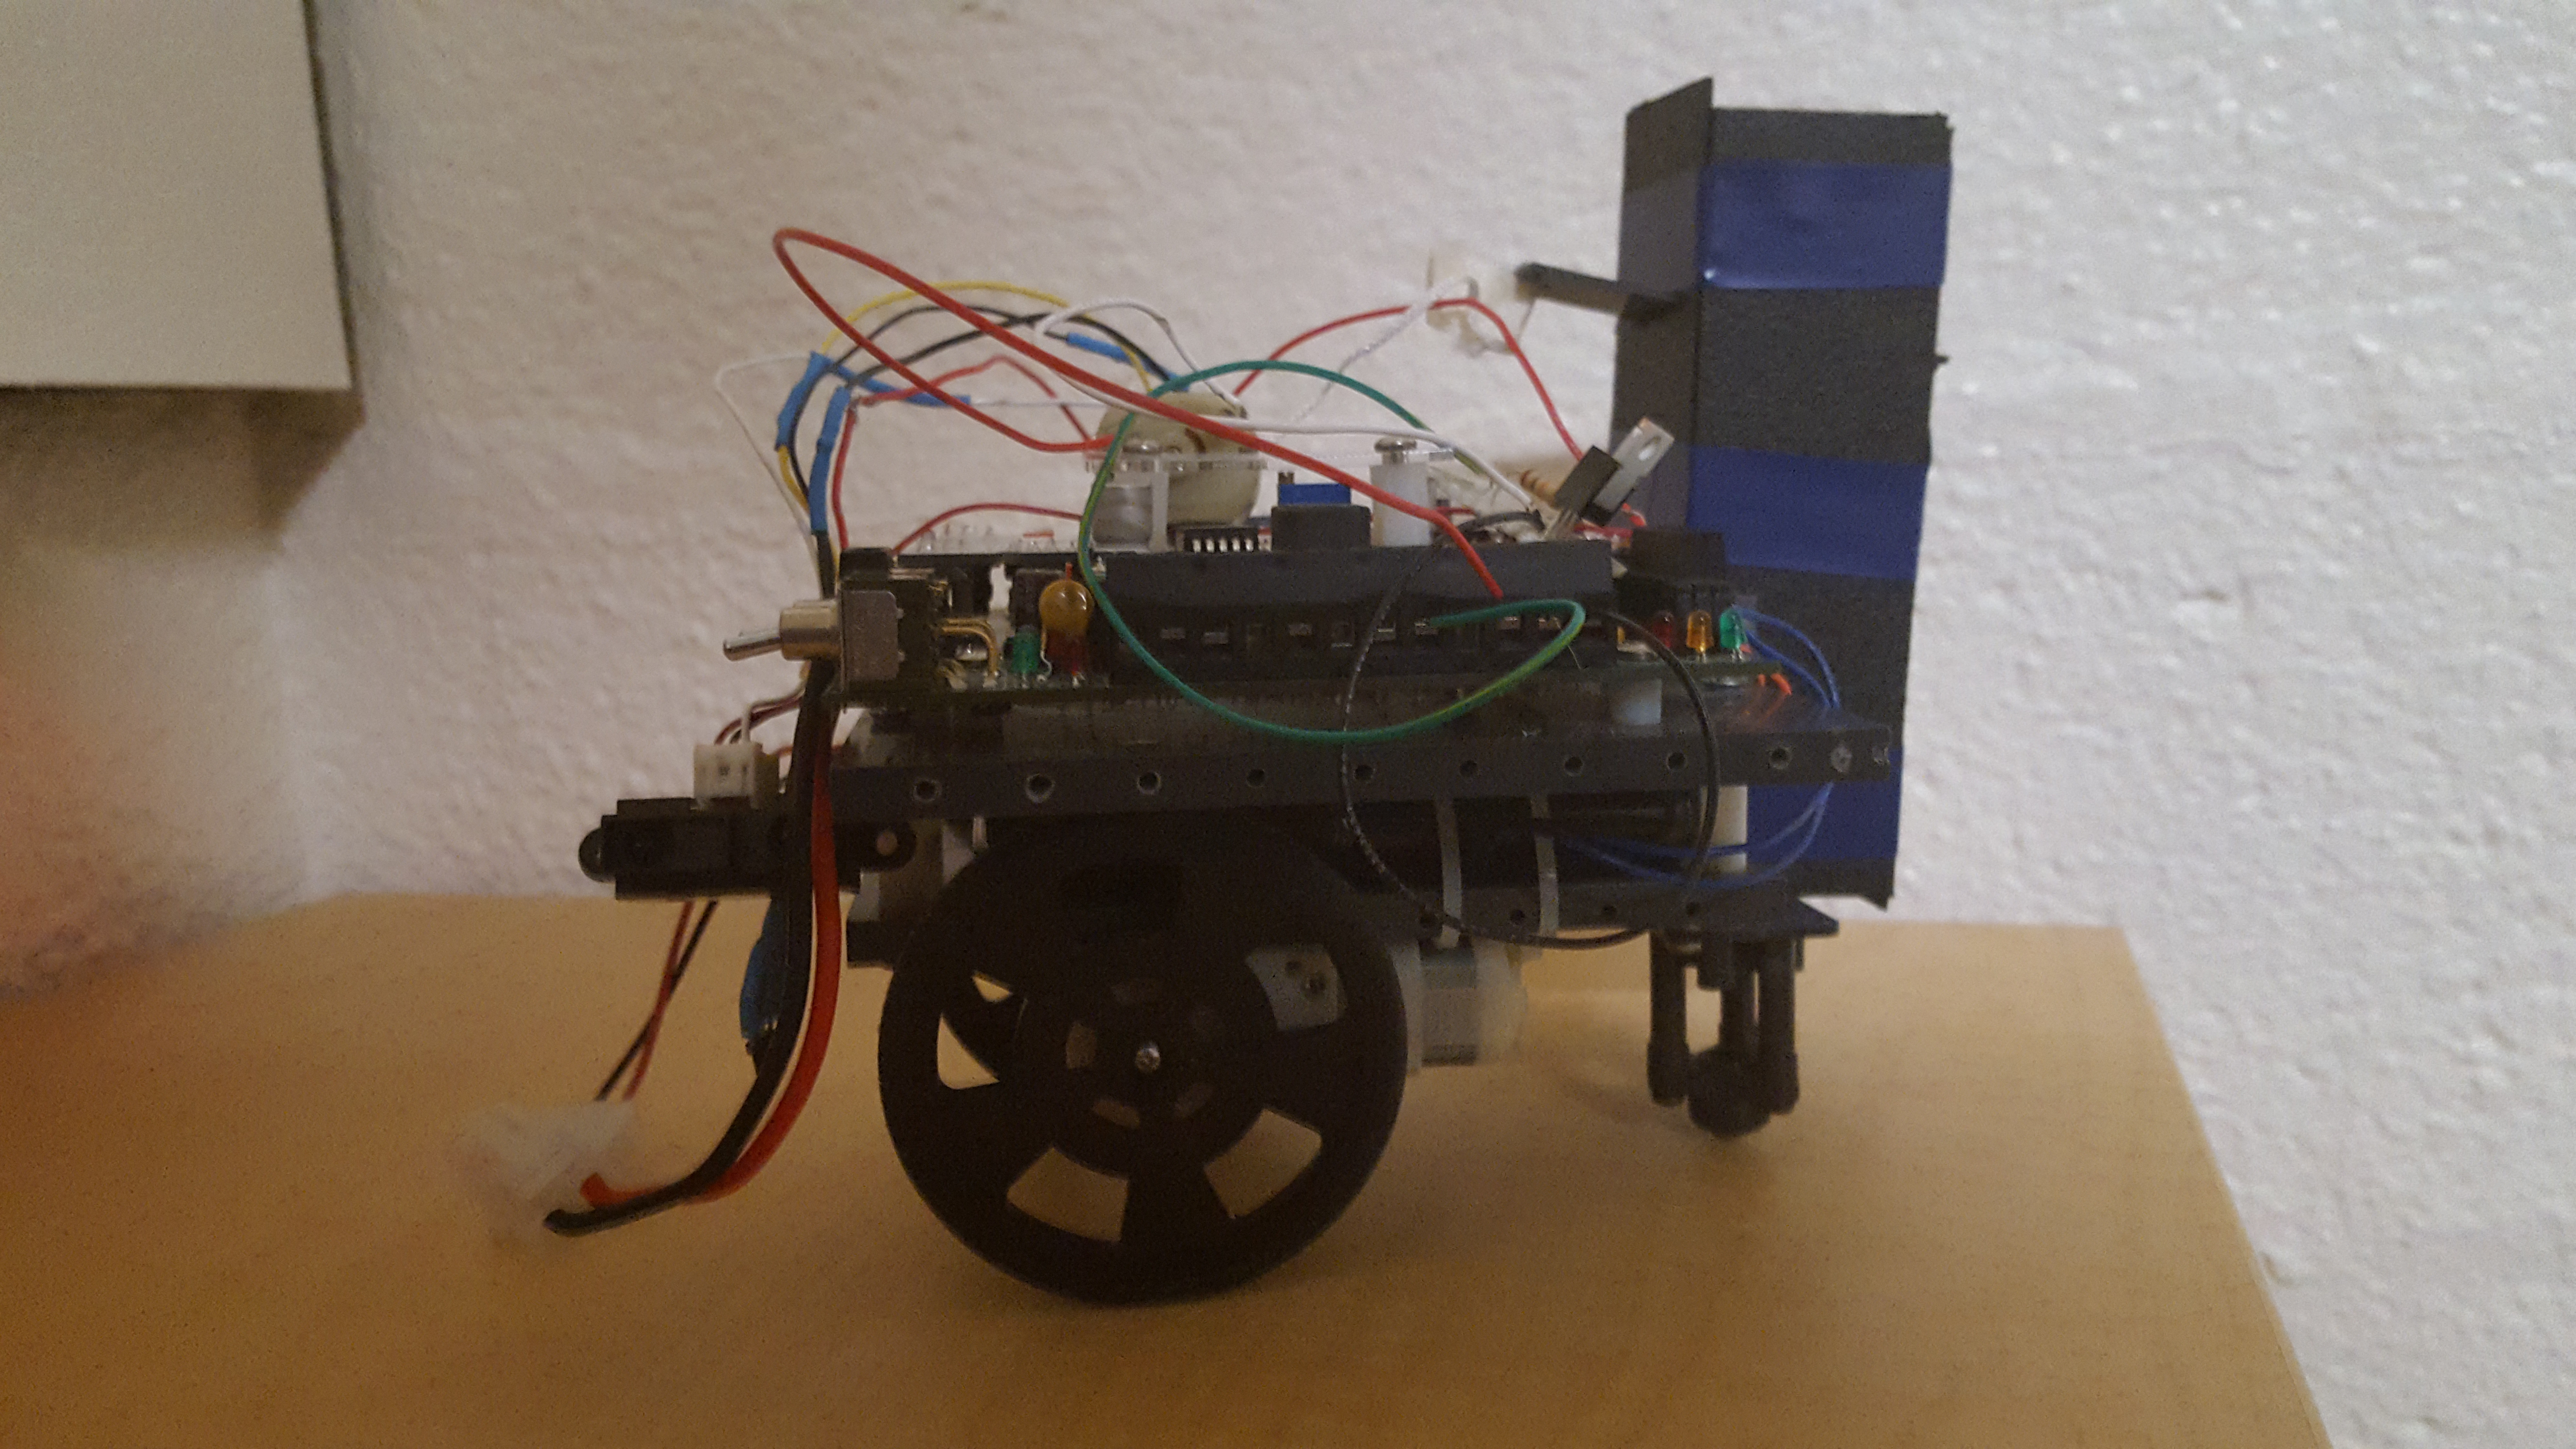
\includegraphics[width=\textwidth]{RobotSide.jpg}}\end{center}

\subsection{Figure 10: Robot Top}
\begin{center}{ 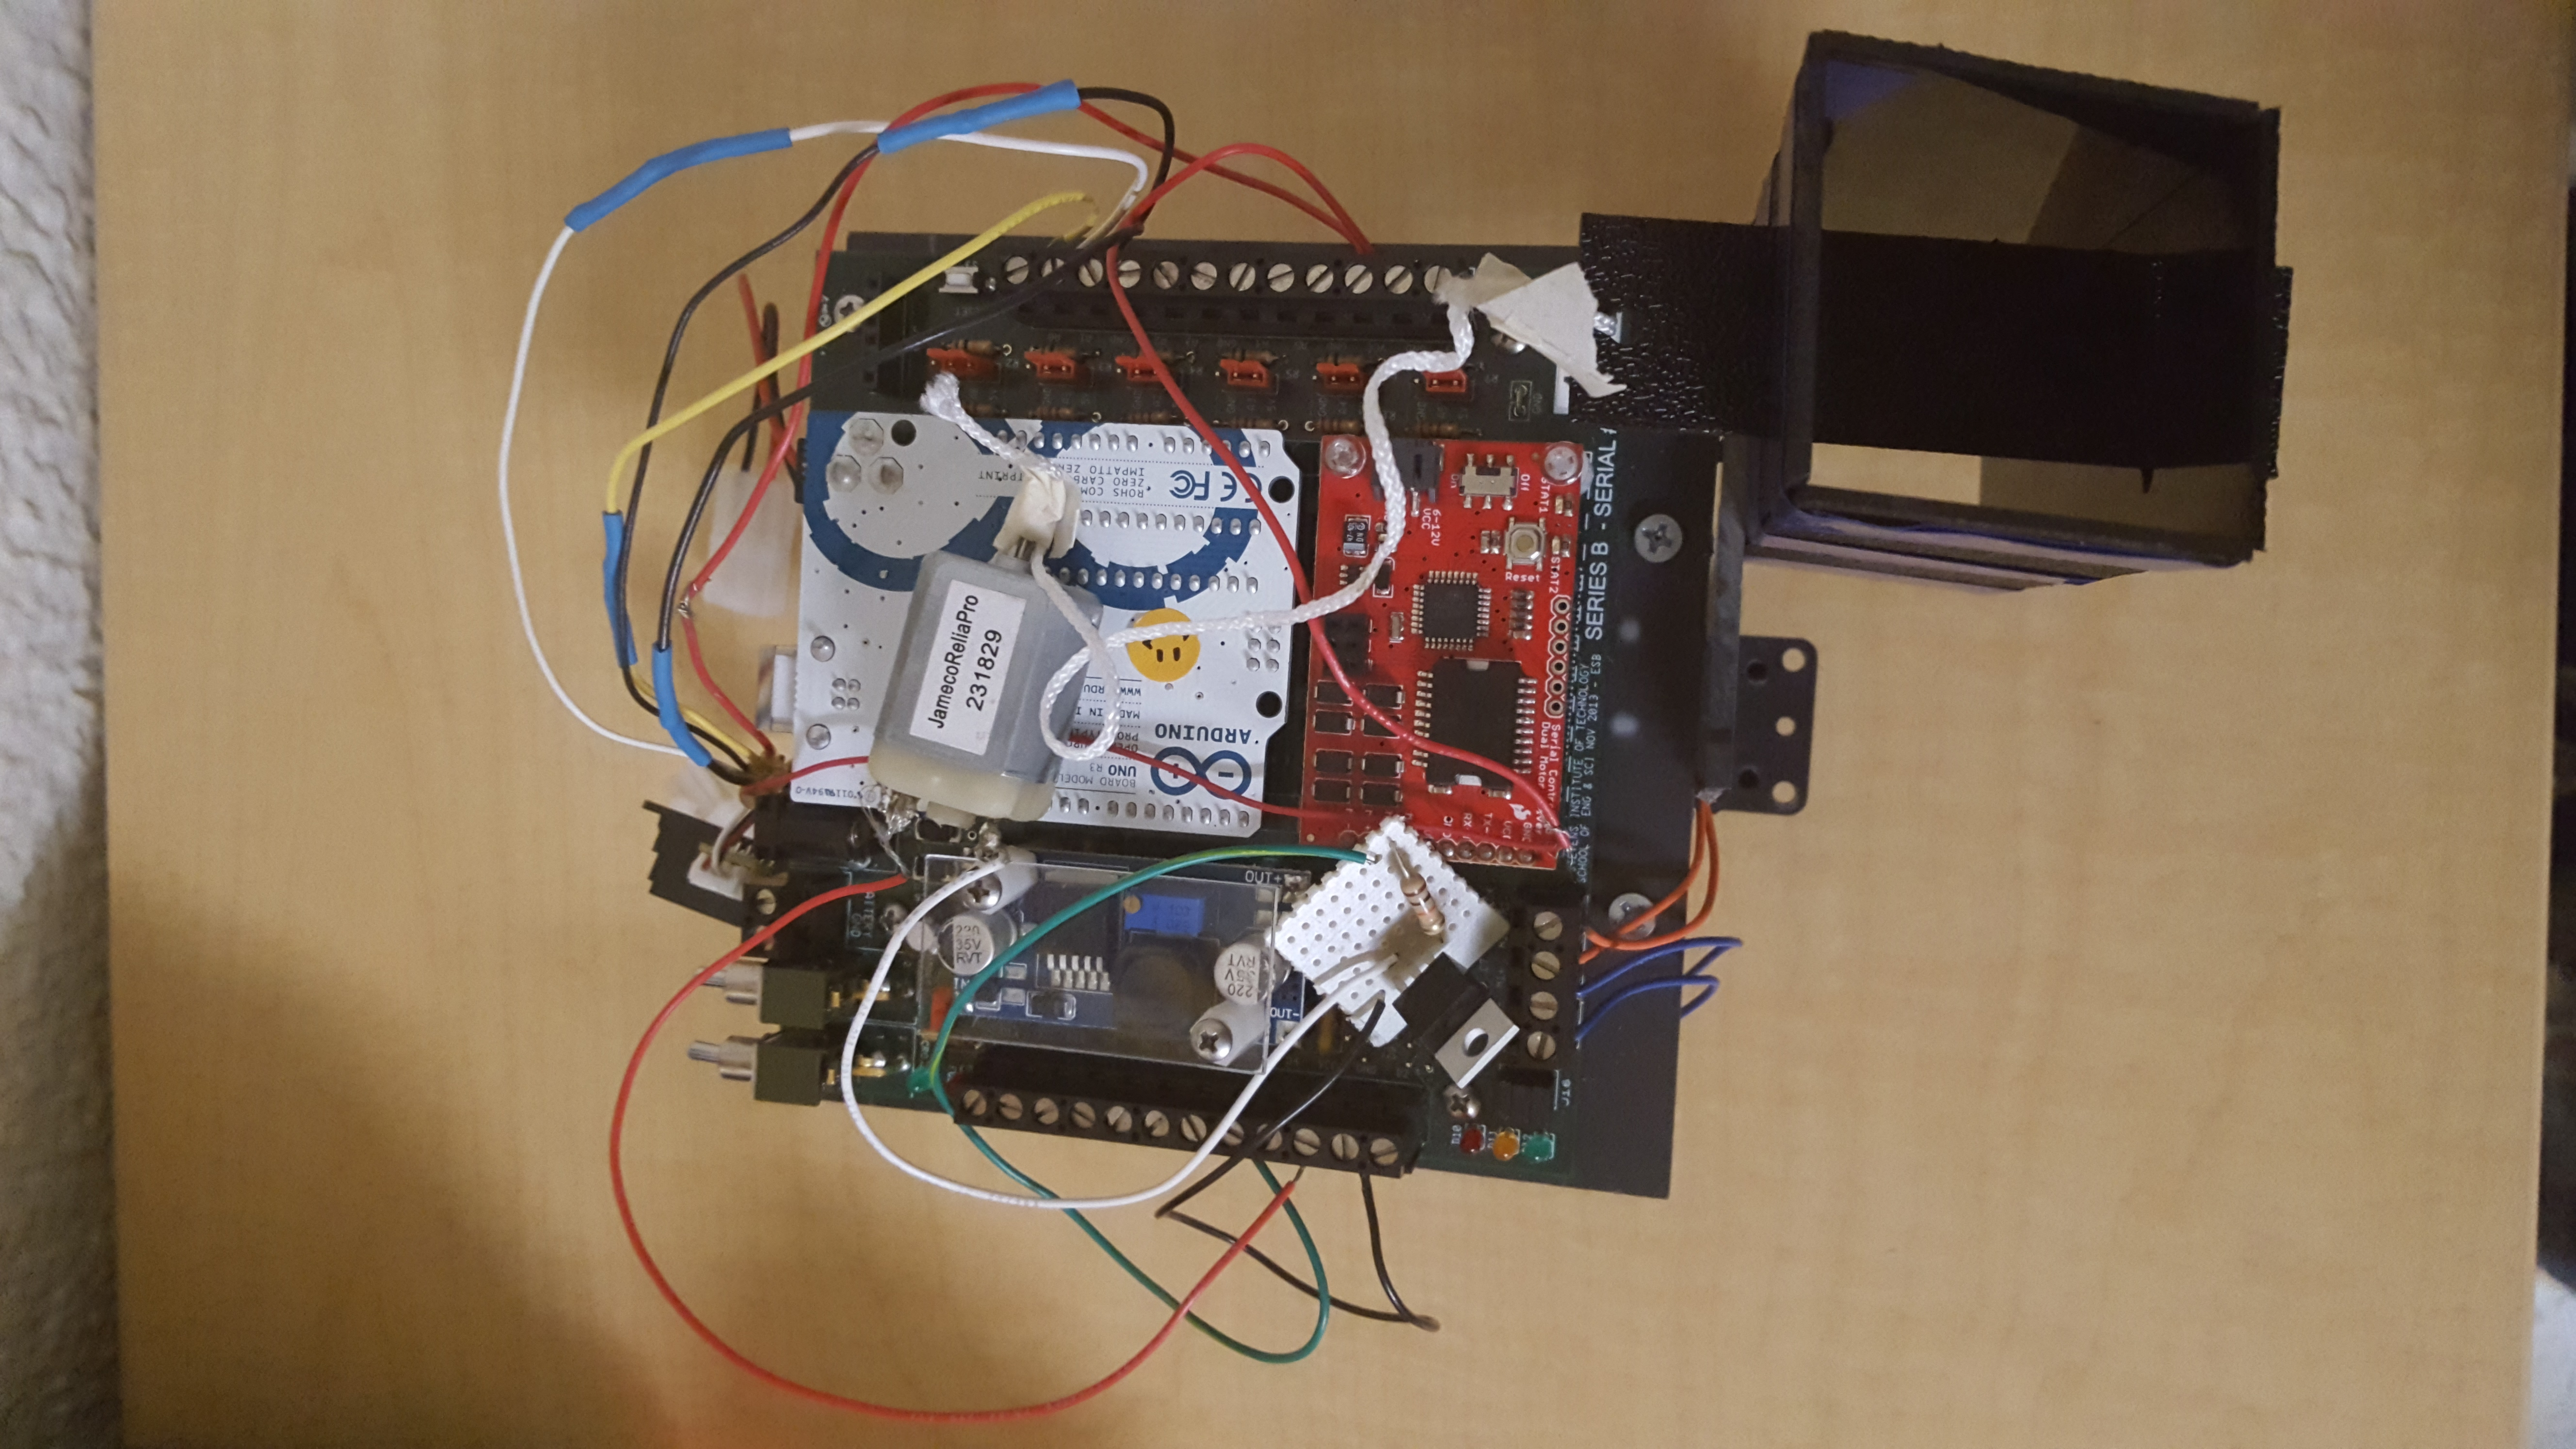
\includegraphics[width=\textwidth]{RobotTop.jpg}}\end{center}

\subsection{Figure 11: Data Flow Chart}
\begin{center}{ 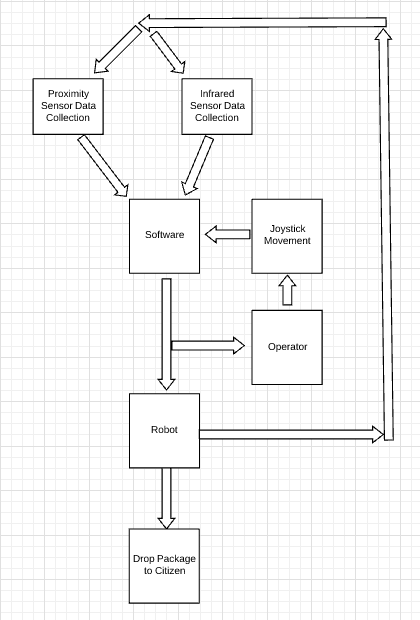
\includegraphics[height=15cm]{DataFlow.png}}\end{center}

\subsection{Figure 12: Software Flowchart}
\begin{center}{ 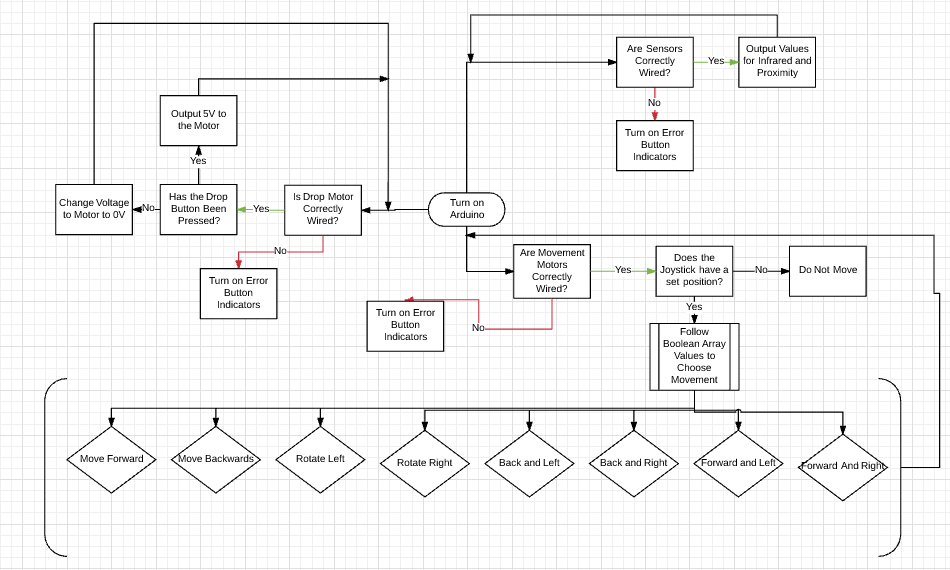
\includegraphics[width=\textwidth]{SoftwareFlowchart.png}}\end{center}

\subsection{Figure 13: Front Panel}
\begin{center}{ 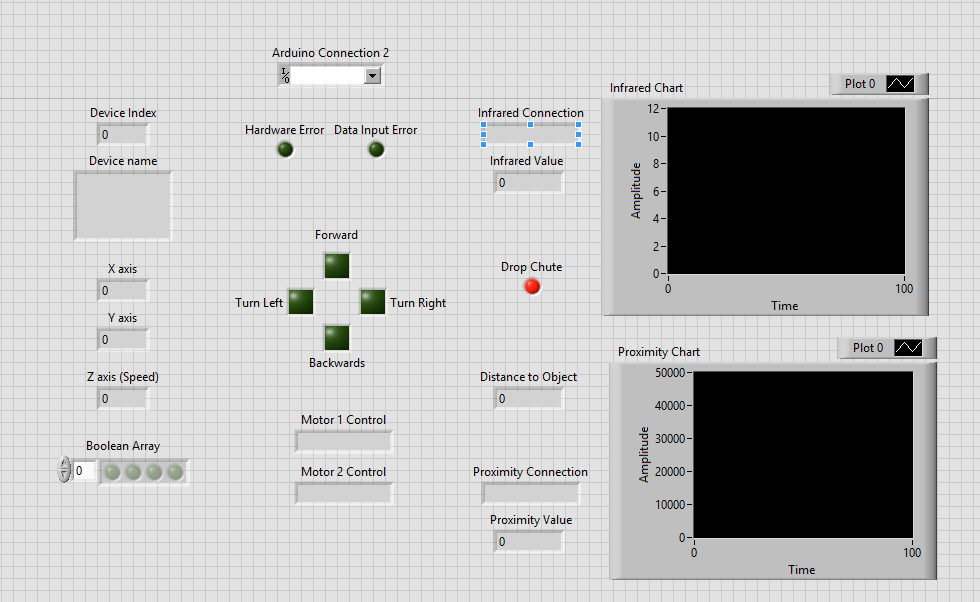
\includegraphics[width=\textwidth]{FrontPanel.png}}\end{center}

\subsection{Figure 14: Joystick VI}
\begin{center}{ 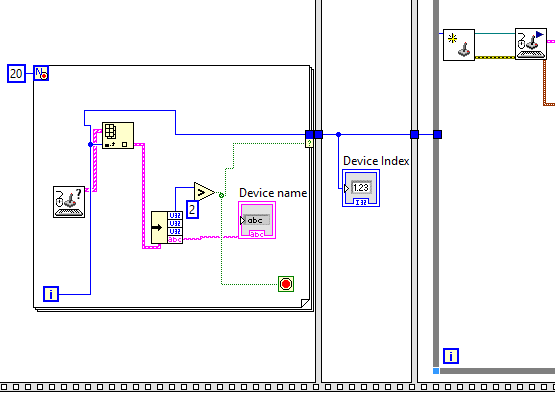
\includegraphics[width=\textwidth]{JoystickVI.png}}\end{center}

\subsection{Figure 15+16: Drop Chute}
\begin{center}{ 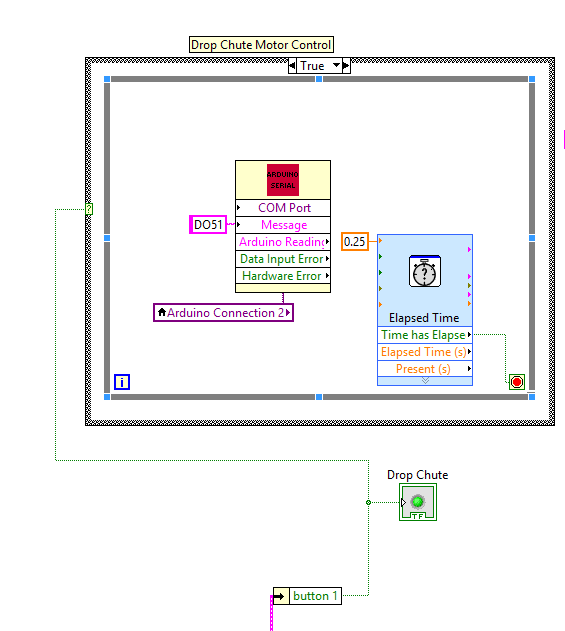
\includegraphics[width=\textwidth]{DropChute1.png}}\end{center}
\begin{center}{ 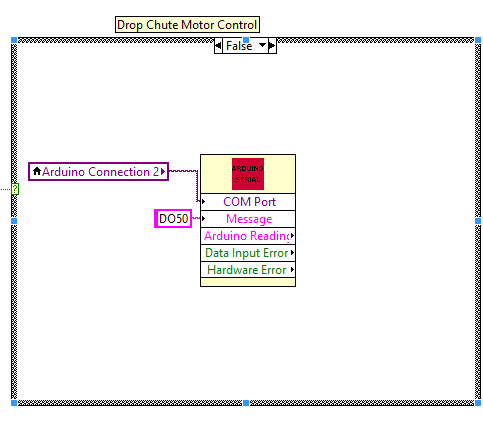
\includegraphics[width=\textwidth]{DropChute2.png}}\end{center}

\subsection{Figure 17: InfraRed Code}
\begin{center}{ 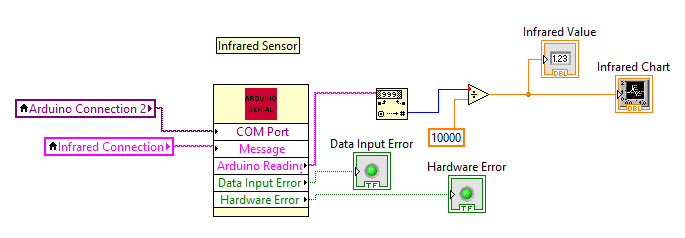
\includegraphics[width=\textwidth]{InfraRedSensor.png}}\end{center}

\subsection{Figure 18: Proximity Code}
\begin{center}{ 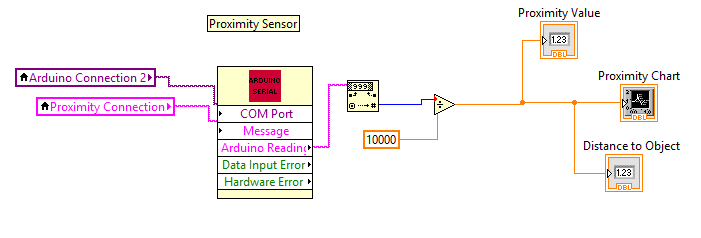
\includegraphics[width=\textwidth]{ProximitySensor.png}}\end{center}

\subsection{Figure 19: Motor Movement Code}
\begin{center}{ 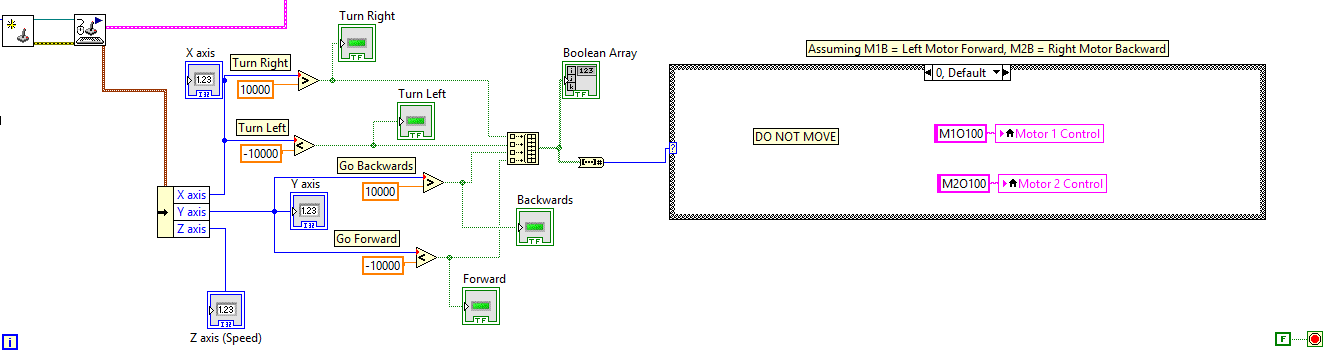
\includegraphics[width=\textwidth]{MotorMovement.png}}\end{center}

\subsection{Figure 20: All Cases}
\begin{center}{ 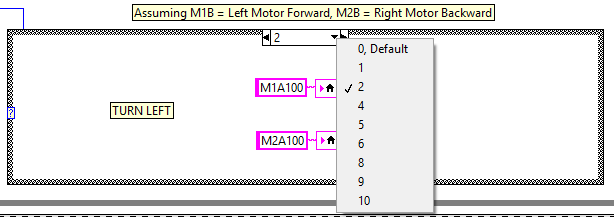
\includegraphics[width=\textwidth]{CaseState.png}}\end{center}

\subsection{Figure 21: Full Code}
\begin{center}{ 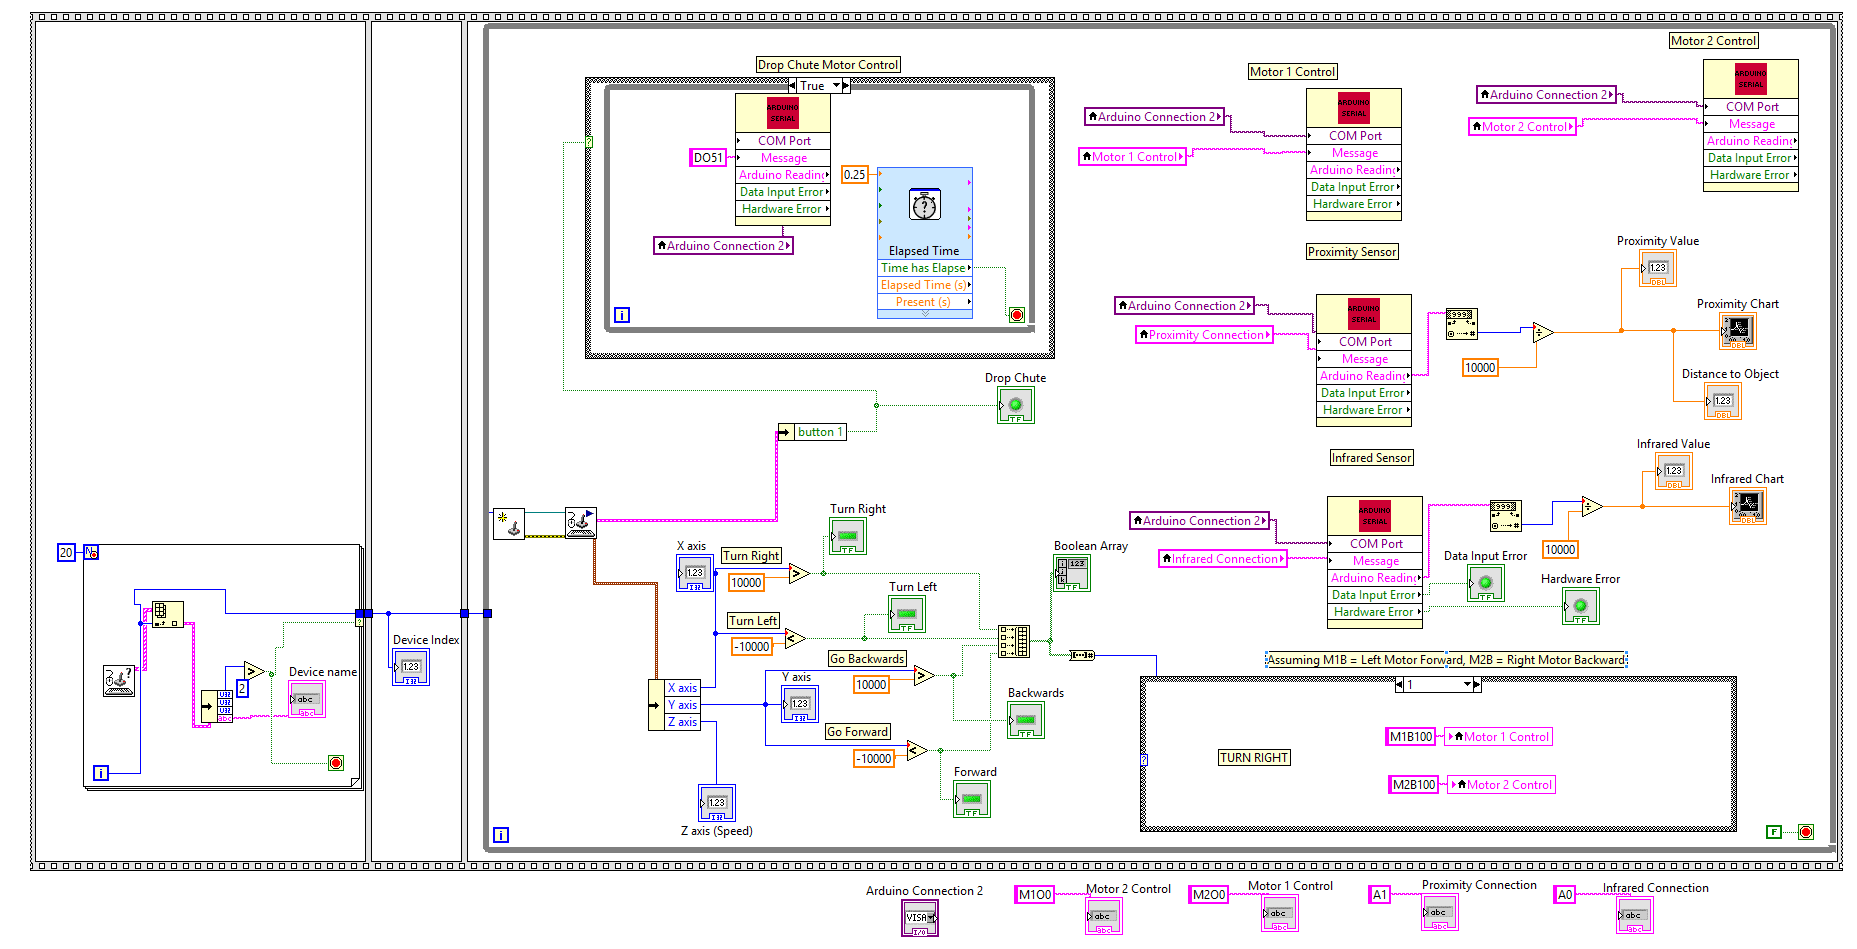
\includegraphics[width=\textwidth]{FullCode.png}}\end{center}

\subsection{Figure 22: Gantt Chart}
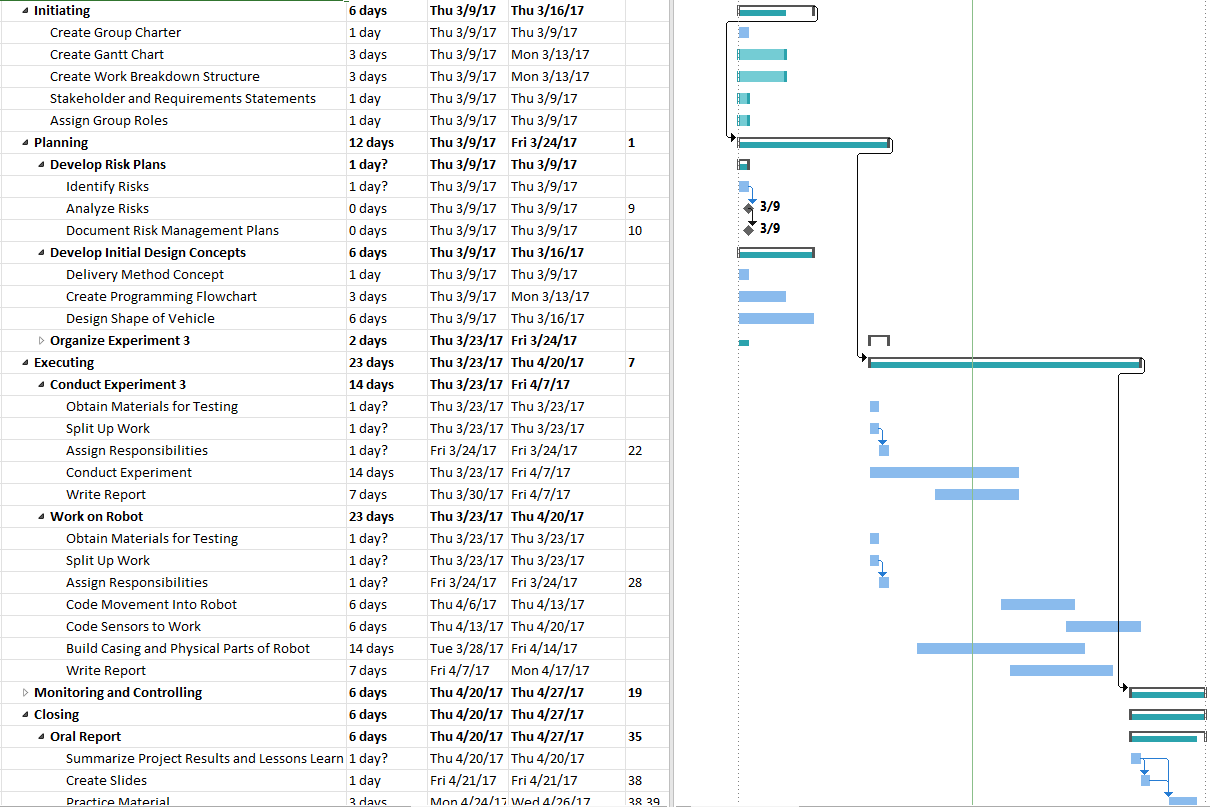
\includegraphics[width=\textwidth]{GanttChart.png}

\subsection{Figure 23: Work Breakdown Structure}
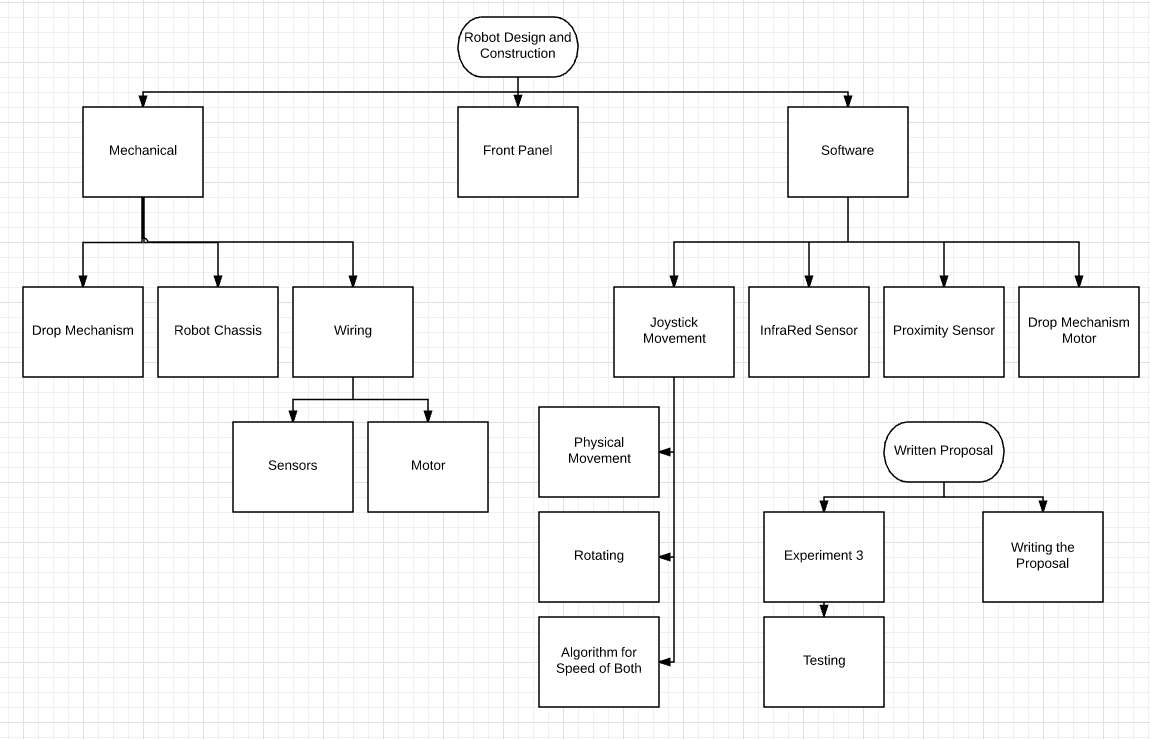
\includegraphics[width=\textwidth]{WorkBreakdown.png}

\subsection{Figure 24: Team Charter}
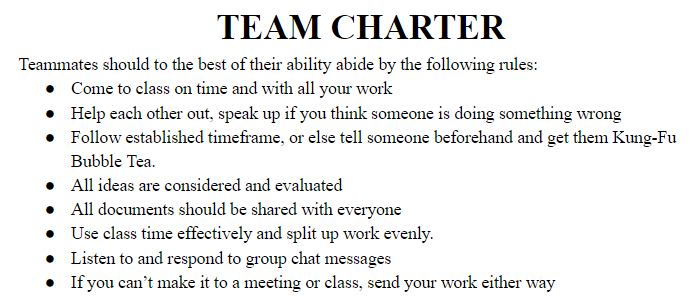
\includegraphics[width=\textwidth]{TeamCharter.png}

\subsection{Figure 25: Financials}
\begin{center}{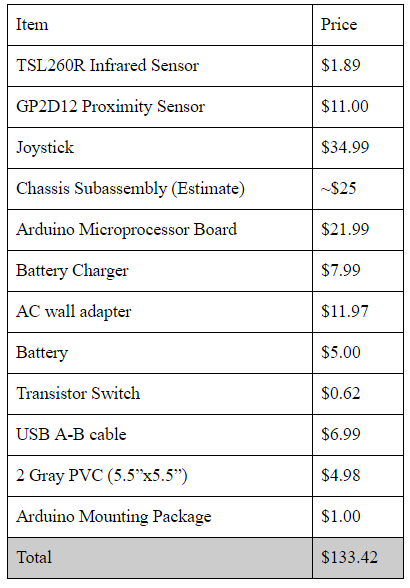
\includegraphics[]{Financials.png}}\end{center}


\end{document}
